
%%%%%%%%%%%%%%%%%%%% file CSMC_MUME_LaTeX_Template.tex %%%%%%%%%%%%%%%%%%%%%
%
% This is the LaTeX source for the instructions to authors using
% the LaTeX document class 'llncs.cls' for contributions to
% the Journal of Creative Music Systems.
% Copyright: http://www.springer.com/lncs       Springer Heidelberg 2006/05/04
%
% It may be used as a template for your own input - copy it
% to a new file with a new name and use it as the basis
% for your article.
%
% NB: the document class 'llncs' has its own and detailed documentation, see
% ftp://ftp.springer.de/data/pubftp/pub/tex/latex/llncs/latex2e/llncsdoc.pdf
%
%%%%%%%%%%%%%%%%%%%%%%%%%%%%%%%%%%%%%%%%%%%%%%%%%%%%%%%%%%%%%%%%%%%
\newcommand{\decfirst}{\textit{Decision.1}}
\newcommand{\decsecond}{\textit{Decision.2}}

\documentclass[runningheads,a4paper]{llncs}
\usepackage{amssymb}
\setcounter{tocdepth}{3}
\usepackage{graphicx}
\usepackage{url}
\usepackage{apacite}
%added 
\usepackage[inline]{enumitem}    
\usepackage{subcaption}
\usepackage{caption}
\usepackage{threeparttable} %annotations for table
\usepackage{csquotes}
\usepackage[title]{appendix}
\usepackage{comment}
\usepackage{multirow}
\usepackage[T1]{fontenc}
\usepackage[bottom]{footmisc}
\usepackage{makecell}
\usepackage{xcolor}

\newcommand{\keywords}[1]{\par\addvspace\baselineskip
\noindent\keywordname\enspace\ignorespaces#1}

\pagestyle{headings}

\begin{document}

\mainmatter  

% AH: If I commented it out, I think it's not great
% AH: Please choose one
% \title{Percussive Sound Generation with Virtual Listeners and Modular Synthesizers}
\title{Percussive Synthesizer Generation with Virtual Listeners}
\title{Percussive Synthesizer Program Generation with Virtual Listeners}
\title{Generating Percussive Synthesizer Programs with Virtual Listeners}
% \title{Listening to generative percussive synthesizer with virtual listeners}
\title{Virtual Listeners to classify Percussive Synthesizer Programs}
\title{Percussion program generation and filtering with Virtual Listeners}
\title{Filtering generated percussion programs with Virtual Listeners}
\title{Listen to it: Generating and filtering synthesizers by percussive qualities}
\title{Virtual Listeners that filter percussion synthesizers}
\title{Generating Drum synthesizers with virtual listeners}
\title{Make your own audience, virtual listeners can filter generated drum programs}
\title{Using AI to filter through millions of synthesizer programs to find some drums}
\title{Finding the drum in the haystack: Using AI Listeners to filter through millions of generated drums}
\title{Program Generation and AI listeners to search for drum synthesizers}
\title{Intersecting AI listener and program generation to find drum synthesizers}
\title{Percussive Synthesizer Program Generation via AI Listening}
\title{Make Your Own Audience: Virtual Listeners Can Filter Generated Drum Programs}



\titlerunning{Make Your Audience}
\author{Amir Salimi \and Abram Hindle}
\authorrunning{Amir Salimi and Abram Hindle }
\institute{Department of Computing Science\\ University of Alberta \\ \email{asalimi@ualberta.ca\\hindle1@ualberta.ca}}


\maketitle

\begin{abstract}
Can we generate drum synthesizers automatically?
We present an approach for the automatic generation of synthesizer programs for one-shot percussive sounds. 
Recent advancements in digital synthesis, heuristic search, and neural networks can be utilized for sound generation. 
Yet the need for data, the problem of open set recognition, and high computational costs persist as barriers towards the expansion of sound libraries using these techniques. 
We generate quick, scalable, percussion synthesizers using classical signal processing. 
We train drum classifiers to find and classify synthesizer programs that mimic percussive sounds. 
We use features from Fourier transformations and autoencoder embeddings to train machine learning classifiers.
Manual listening tests of the generated sounds demonstrates the system can successfully generate drum synthesizers and categorize drum sounds.
To facilitate future research, we share our curated dataset of free percussive sounds.
\keywords{Automatic Synthesizer design. Machine Listening. Sound Analysis. Novelty and Originality}
\end{abstract}


\section{Introduction} 
Digital recordings of novel, one-shot\footnote{A single hit on the drum that captures its capabilities} drum sounds are commonly used in  electronic music compositions. Yet unique drum sounds can be difficult or expensive to find. By relying on recordings of material drum sounds, artists are limited by what instruments exist in the material world and whether or not high-quality, one-shot recordings can be accessed. We believe automatic programming of virtual synthesizers for the creation of novel drum sounds can alleviate these limitations. To this end, we implement a programmable virtual synthesizer of audio, which we call the \emph{virtual synthesizer}. We also implement machine learning classifiers for automatic separation of percussive sounds from non-percussive sounds. To effectively train the classifiers with small datasets, we simplify the representation of audio data by experimenting with fast Fourier transforms (FFT) and autoencoder embeddings. We call our system of feature extraction and classification of sounds the \emph{virtual ear}. To create a dataset of synthetic drums, the virtual synthesizer produces random programs and generates the corresponding audio. This audio is then categorized by the virtual ear. We save not just the desirable sounds, but also the programs which generated these sounds, which can be modified and experimented on by sound designers. In this work, only random search is used for program generation, but other heuristics can be integrated for an improved search algorithm in future works. We build generative systems using different implementations of the virtual ear, and conduct manual, blinded hearing tests of the generated sounds. Our results are promising as the majority of sounds generated from our systems are deemed percussive by human listeners. However, we cannot quantify the novelty of these sounds. 
 \begin{figure}[tb]
    \begin{center}
    % \textbf{Generative System}
    \makebox[\textwidth]{
    \fbox{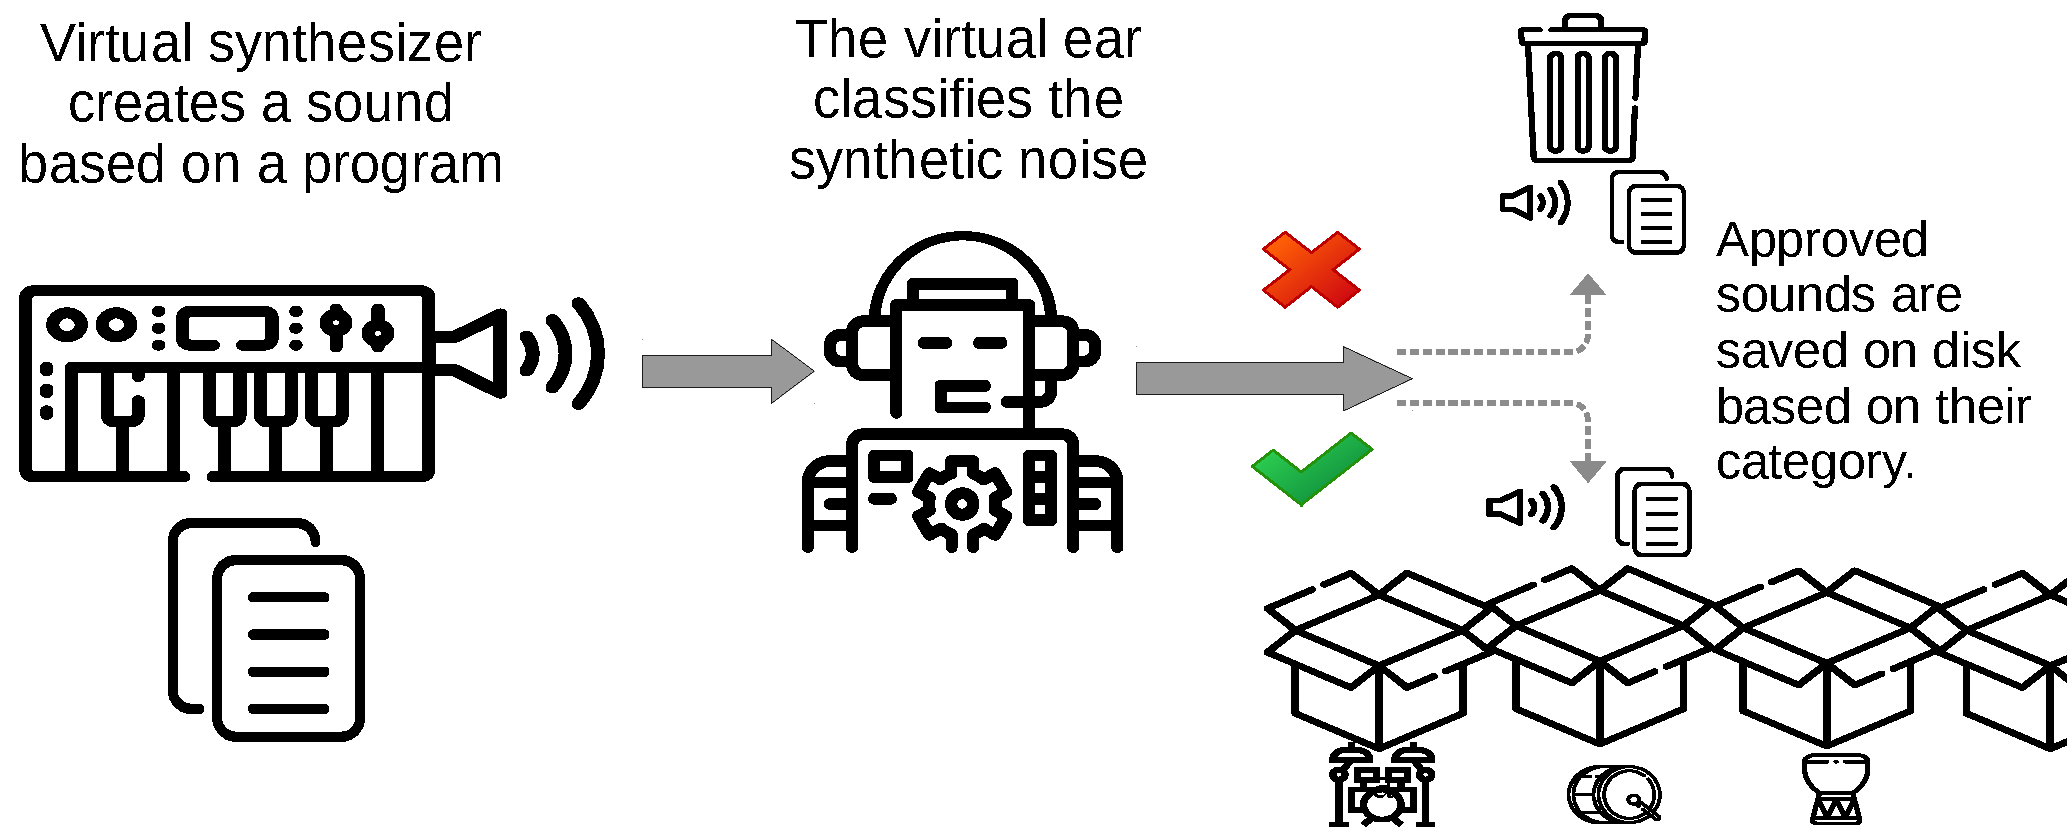
\includegraphics[width=1\linewidth]{images/pipeline.pdf}}}
    \end{center}
    \caption{A blueprint of our system which allows each component to be implemented in a number of ways. Our implementations of this pipeline allow for easy parallelization when needed. This implementation also allows for easy integration of heuristic search for future works. 
    }
\label{fig:pipeline_outline}
\end{figure}

\begin{table}[tb]
\centering
\caption{Curated databases}
\begin{tabular}{ |c|c| } 
\hline
DB Name & Categories                                                        \\ \hline
FreeDB  & Kicks:533 - Snares:372 - Claps:230 - Hats:105 - Other:281            \\ \hline
RadarDB & \makecell{Kicks:1054 - Snares:842 - Claps:353 \\ Toms:349 - Hats:1561 - Rims:131 - Shakers:121} \\ \hline
MixedDB & Kicks:533 - Snares:372 - Claps:230 - Hats:105 - Others:281                     \\ \hline
% NoiseDB & Generatable      & 1 Stack:2000 3 Stacks:2000  5 Stacks:2000                         \\ \hline
\end{tabular}
    % \caption{Overview of our datasets.}
    \label{table:drumdb}
\end{table}

% \section{Datasets}

Furthermore, we provide a subset of our curated datasets to facilitate future research. We curated 3 datasets of one-shot drums which we use to train and validate drum classifiers. The number of samples per group in these databases is provided in Table ~\ref{table:drumdb}. We provide unrestricted access to \textbf{FreeDB} via Zenodo\footnote{\url{https://zenodo.org/record/3994999}}.
\textbf{RadarDB} cannot be shared directly, we provide the script for its automated creation\footnote{\url{https://github.com/imilas/Synths_Stacks_Search}}. We cannot provide a copy of \textbf{MixedDB}, which is curated from various sources and personal libraries. 
 % \section{Datasets}
% We curated 3 data-sets of one-shot drums which we use to train drum classifiers. \textbf{FreeDB} contains 5 categories: kicks, snares, claps, hats and other (various percussions). \textbf{RadarDB} contains 7 categories: kicks, snares, claps, hats, shakers, toms and rims. \textbf{MixedDB} contains 8 categories: kicks, snares, claps, high toms, low toms, medium toms, closed hats and open hats. See Appendix~\ref{appendix:datasets} for details and download links.   
\section{Related Works}
Numerous deep neural network models have been proposed for the purpose of signal generation in recent years~\cite{nsynth2017,yamamoto2020parallel,oord2017parallel,yee2018automatic,ramires2020neural}. WaveGans and WaveNet have been subject to significant improvements and experiments since their proposal~\cite{nsynth2017,yamamoto2020parallel,oord2017parallel}. Particularly relevant works are the utilization of variational autoencoders (VAE's) for generation of percussive samples~\cite{aouameur2019neural} and generation of percussive sounds by decoding a small set of latent features~\cite{ramires2020neural}. Automatic programming~\footnote{unsupervised generation of source code or programs towards a goal} of virtual synthesizers has long been a topic of interest. Genetic Algorithms (GA's) have been utilized for the generation of new sounds with various sound engines~\cite{hornermachinetongues,macret2012automatic}. A more recent work by Yee-King et al.~\cite{yee2018automatic} used Long short-Term Memory (LSTM) models and heuristic search to find the exact parameters used to create a group of sounds. The sounds approximated were made by the same virtual synthesizer and not with an external source. Esling et al. used  over 10,000 VST synthesizer presets to learn a parameter space which can be sampled for creation of new audio~\cite{esling2019universal}. Here, we work towards the approximation of percussive sounds with no prior knowledge about the parameter space of a synthesizer.

\section{Virtual Synthesizer Design}
\begin{table}[tb]
\centering
\caption{Synthesizer submodule parameters. $10^{15}$ unique programs are possible. Each synthesizer can contain any number of submodules}
\resizebox{\columnwidth}{!}{\begin{tabular}{ |>{\centering\arraybackslash}p{4cm}|>{\centering\arraybackslash}p{4cm}|>{\centering\arraybackslash}p{4cm}| } 
\hline
Parameters & Value Range & Notes and Constraints\\
\hline \hline
Attack & 0-3 & A-D-S-R values relative\\
Decay & 0-3 & relative to A-S-R\\
Sustain & 0-3 & relative to A-D-R\\
Release & 0-3 & relative to A-D-S\\
OSC type & sine,square,saw & -\\
IsNoise & boolean & generate noise using \newline cloud of waveform\\
Length & 0-1 second & - \\
StartTime & 0-1 second & Length+Start$<$1\\
Amplitude & 0.1-1 & 1 = max amplitude\\
Pitches(notes) & list of pitches &  range of C0(16.35hz) to B9 \\
HP filter Cutoff & 0-20000hz & -\\
LP filter Cutoff & 20000hz-HP & never lower than HP cutoff\\
Filter Order & 4,8,16 & butterworth filter order \\
\hline
\end{tabular}}

\label{table:submodule_params}
\end{table}
To create sounds, we build digital synthesizers. We use classical DSP to build our synthesizer, which allows for quick, offline, and parallel generation of audio signals without the usage of GPUs. We made extensive use of Pippi\footnote{https://github.com/luvsound/pippi} and SciPy~\cite{jones2001scipy} libraries. Our virtual synthesizer contains a set of one or more submodules. Each submodule is a self-contained noise making unit and creates signals by taking the steps depicted in figure~\ref{fig:submodule}. Submodules have identical sets of parameters, but widely different outputs can be achieved depending on the values assigned. The set of required parameters for each submodule is highlighted in Table~\ref{table:submodule_params}. The sonic output of the virtual synthesizer is the normalized addition of the output of its submodules. Our implementation of a synthesizer can have any number of submodules. We call the number of submodules in each virtual synthesizer the \textit{stack size}. We call the sets of parameter values that characterize a synthesizer's submodules a \textit{program}(analogous to presets and submodules for a VST).  
 \begin{figure}[tb]
    \begin{center}
    % \textbf{Synthesizer SubModule }
    \makebox[\textwidth]{
    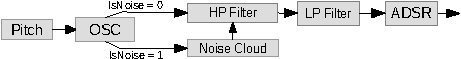
\includegraphics[width=1\linewidth]{templates_aimusic2020/images/synthesizer_block_thin.pdf}}
    \end{center}
    \caption{High level representation of pre-rendering steps for each submodule. Each Synthesizer contains 1 or more these submodules. Synthesizer programs set the number of these submodules and their parameters. The output of a synthesizer is the normalized addition of all its submodule outputs. 
    }
\label{fig:submodule}
\end{figure}
 Rather than directly using neural networks for sound synthesis, we generate programs for this virtual synthesizer. Our decision is based on the following factors:
\begin{enumerate*}[label=(\roman*)]
    \item \textit{Novelty and Creativity}: The goal here is to work with the limitations of any tractable sound source to create its approximations of a given sound category. We seek to create novel sounds via artificial, exploratory creativity. Boden defines this concept as an emergent property of generative work within confined rule sets~\cite{boden2009computer}. An example is the perpetual popularity of 8-bit aesthetics~\cite{collins2007loop}. 
    \item \textit{Interpretability}: Neural networks are often described as black boxes with uninterruptible weights~\cite{basheer2000artificial}. Their highly recursive structure makes modern explanation methods such as saliency maps unreliable~\cite{rudin2019stop}.  
    \item \textit{Speed of Rendering}: Neural network synthesis is costly; Sub 24 khz sample rates are common in most relevant works~\cite{yamamoto2020parallel,oord2017parallel,aouameur2019neural,ramires2020neural}. This is far below CD quality sampling rates~\cite{reiss2016meta}. At our fixed sampling rate of 48 khz, synthesizers with 8 submodules can create and save 1 second sounds to hard-disk with an average rendering time of 50 milliseconds\footnote{Using a single process on a Macbook Air 2012 and Ubuntu 18.04}. 
    \item \textit{Flexibility and Scaling}: Probabilistic audio generation is often done sequentially. State of the art, parallel wave generation with GANs requires a fixed amount of rendering time for each time-step~\cite{yamamoto2020parallel}. With our virtual synthesizer, the added footprint of increasing the length of rendered sounds or higher sampling rates is relatively minuscule.  
\end{enumerate*}

%  Evaluation of a periodic function such as sine or cosine is the simplest form of software audio generation~\cite{mitchell2009basicsynthChap5}. This generative system is called an \textit{oscillator}. With careful programming, DSP techniques can be used to replicate almost any sound~\cite{jenkins2019analog}. Synthesizers we build using these functions are tractable and explainable: the output is determined by the input and reproducible. This makes the evaluation of a set of inputs (or parameters) to our synthesizers relatively simple.
 

\section{Virtual Ear}
\label{section:virtual_ear}
The virtual ear receives sounds and discards those which do not resemble drums. It then classifies sounds by drum category. Our goal is to produce a virtual ear that accurately discriminates between percussive and non-percussive sounds, but is tolerant of novelty. The virtual ear makes two critical decisions: 
\emph{
\begin{quote}
\text{Decision.1 Could the sound be used as a drum?}
\\
\text{Decision.2 If it does sound like a drum, what type of drum should it be?}
\end{quote}
 }
 \begin{figure}[tb]
    \begin{center}
    \makebox[\textwidth]{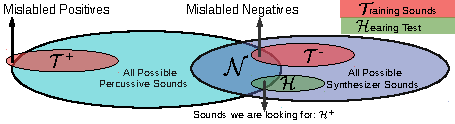
\includegraphics[width=0.95\linewidth]{images/venn_data.pdf}}
    \end{center}
    \caption{ An illustration of the discrepancy between the sounds we use to train our classifiers and the type of sounds the classifier is expected to classify. $\mathcal{N}$ is the set of percussive sounds a synthesizer is capable of making. The inclusion of sounds in this group may vary from person to person. Our positive samples, $\mathcal{T^{+}}$, is a small fraction of a wide variety of percussive sounds that are conceivable. For $\mathcal{T^{-}}$, we can generate any number of random samples. $\mathcal{H}$ is a series of sounds sent to the ear for classification.
    }
\label{fig:ven_data}
\end{figure}
\decfirst~requires knowledge of what drums \textbf{do not} sound like, or knowledge of an infinitely large set, which cannot be fully represented via examples. An important consideration is that the source of sounds used for training the model (organic drum sounds) will be fundamentally different from the source of unlabeled sounds we wish to categorize (noise from a synthesizer). This issue is reflective of the open set recognition (OSR) problem~\cite{geng2020recent,mundt2019open}. We use Figure~\ref{fig:ven_data} to highlight a number of caveats with our training approach. If the sound is deemed percussive, the virtual ear makes \decsecond~by finding the best drum category for the sound. The number of categories available is dependent on the database of drums used for training. 
To maximize the transference of knowledge gained from training the classifiers to evaluation of programs, we need to extract concise feature sets that capture fundamental characteristics of the data points.\\

In order to classify sounds, we need to summarize them as features. Various works have demonstrated effective reconstruction of signals given their Short-time Fourier Transforms (STFT)~\cite{nawab1983signal,griffin1984signal}. If the STFT of a signal can be used for its reconstruction, perhaps it can be utilized as a source of fundamental features~\cite{lee2009unsupervised,huzaifah2017comparison}. We defined 3 STFT (or FFT) transformation functions to capture important features of percussive sounds. 
\begin{enumerate}
\item Envelope Transformation: Represents changes in loudness for the duration of the signal. Using STFT we generate a matrix $M_{i \times j}$ with rows $i$ and columns $j$ corresponding to time steps and frequency bins. Values $v_{i \times j}$ indicate the magnitude of frequency bin $j$ at each time-step $i$. We approximate the envelope of the signal by summing the values of $M$ at each time-step. 
\item Frequency Transformation:  Similar to envelope calculation, but the summation is done along the frequency axis. Shorter hop-sizes and wider windows were used to increase frequency resolution. 
\item Spectrum Transformation: Mel Scaled STFT. Values normalized from 0-1. 
\end{enumerate}

Another set of features were extracted using the latent embeddings of autoencoder networks. Here, an autoencoder is a combination of an encoder which encodes spectrograms into a lower dimension and a decoder which tries to decode these embeddings into the original data. We trained a number of autoencoders with spectrogram transformations, and used the encoder from the autoencoder network with the lowest decoding loss as a feature extractor~\footnote{Appendix~\ref{appendix:hyperparam} has further details on the hyperparameter search process}. Latent embeddings at the bottleneck layer of our best spectrogram autoencoder are used as features for sound categorization. 

% \textcolor{red}{ As a sanity check for this approach, we trained our best autoencoder using 80\% of the drums in MixedDB. Latent encodings of the remaining 20\% and 1000 Noise sounds were projected onto a 2 or 3-dimensional planes using t-SNE. We implemented interactions for our projection graphs (see Appendix~\ref{appendix:tsne}) so the sounds associated with plot points can be listened to. Hearing tests revealed a noticeable, positive correlation between a synthetic sound's distance and similarity to drum clusters.}

% Please add the following required packages to your document preamble:
\begin{table}[tb]
\caption{Overview of survey model architectures. Further details in Appendix~\ref{appendix:classifier_definitions}}
\resizebox{\textwidth}{!}{%
    \begin{tabular}{|>{\centering\arraybackslash}p{2cm}|>{\centering\arraybackslash}p{10cm}|>{\centering\arraybackslash}p{2cm}|}
    \hline
    Model & Architecture Layout                                                                             & Features                 \\ \hline
    CNN(TPE)   & CNN(2 channel convolution)~ -\textgreater~LSTM(800 hidden states)~-\textgreater\newline ~Linear Layers (shape 400x5)                                 & Spectrogram          \\ \hline
    FC(TPE)    & Fully connected Linear layers with shape: 400x10x5x10x5                                & Spectrogram          \\ \hline
    E+F(TPE)   & Fully connected network of size 50x10x2x5 & Env. + Freq. \\ \hline
    MEM   & Encoder -\textgreater~Embedded Spectrogram(size 64) -\textgreater~Extra-Trees                                              & Spectrogram          \\ \hline
    \end{tabular}
}
\label{table:brief_models}
\end{table}

To automatically learn from the extracted features, two groups of virtual ears are implemented: \emph{two phased ears} (TPEs) and \emph{Mixed Ear Models} (MEMs).  For TPEs, we train multiple neural network architectures using different subsets of the FFT features to specialize in \decfirst~or \decsecond~and combine them to make decisions sequentially. To train TPEs for \decfirst, we use all drums in RadarDB and FreeDB and 6000 examples of virtual synthesizer noise. For \decsecond, we combine the two databases and merge toms into kicks and rims/shakers into \enquote{other}. We trained the TPE models with 80\% of this dataset. Using the remaining 20\% of sounds, we achieved 98\% accuracy in \decfirst~and 82\% accuracy in~\decsecond~with our best models. These accuracy numbers are weak as we did not account for category sizes or cross validate.

% To automatically learn from the described features, two groups of synthetic ears are implemented: \emph{two phased ears} (TPEs) and \emph{Mixed Ear Models} (MEMs).  We train multiple neural network architectures using different subsets of the FFT features to specialize in \decfirst~or \decsecond~. Our design of TPE ears allows a combination of these networks to make sequential decisions. To train TPEs for \decfirst, we use all drums in RadarDB and FreeDB (categories do not matter). To learn \enquote{not-drums}, TPEs are given 6000 examples of synthesized noise. For \decsecond, we combine the two databases and merge toms into kicks and rims/shakers into \enquote{other}. We designed and trained a number of neural net architectures with 80\% of this dataset. Using the remaining 20\% of sounds, we achieved 98\% accuracy in \decfirst~and 82\% accuracy in~\decsecond. Our best models both utilize convolutional neural net (CNN) layers that learn from spectrogram data. These accuracy numbers are weak as we did not account for category sizes or cross validate.

MEMs learn from autoencoder embeddings and envelope features and give simultaneous answers to both decisions. We use kicks, snares, claps, and hat sounds from RadarDB and FreeDB as well as 1000 examples of synthesized noise to train MEMs. Using 10-fold cross validation, our best MEM (an ExtraTrees Classifier) achieves the average f1-score of 92\% in 5-way sound classification (4 drum categories + synthesized noise). Detailed measurements and model descriptions for TPEs and MEMs can be found in table~\ref{table:brief_models} and Appendix~\ref{appendix:classifier_definitions}. 

\begin{figure}[tb]
\begin{center}
% \textbf{Visual Representation of FFT Features}\par\medskip
    \includegraphics[width=0.99\columnwidth]{templates_aimusic2020/images/ff3.pdf}
\caption{Visualized representation of FFT features for a randomly synthesized noise. More examples in Appendix~\ref{appendix:trans_funcitons}.}
\label{fig:stackspectrums}
    \end{center}
\end{figure}

\section{Building and Evaluating The System}
% Please add the following required packages to your document preamble:
% \usepackage{multirow}

High accuracy in detection of organic drums vs synthetic sounds does not necessarily make an ear more suitable for our generative system. Perfect detection would create a system which generates nothing.  We cannot know the true size of $\mathcal{H^{+}}$ (see Figure~\ref{fig:ven_data}) without exhaustive manual hearing tests. We conduct blinded hearing tests of two generative systems. For \decfirst, a network which learns from spectrogram data utilizing CNN and LSTM layers is used. For \decsecond, we categorize the drum types with 3 different models: FC (Fully-Connected architecture and spectrograms for learning), CNN (CNN and LSTM layers with spectrograms), and E/F (Fully-Connected architecture with frequency and envelope features). The MEM system uses our best MEM, which simultaneously classifies sounds as drums and categorizes them. 

The TPE system produces samples in the following categories: \enquote{snare}, \enquote{kick}, \enquote{hat}, \enquote{clap} and \enquote{other} (combination of rims, shakers and unusual percussive sounds). The MEM system does not output the \enquote{other} category, yet the option is available to surveyors when categorizing sounds manually.   
Both authors categorized a subset of the results without knowledge of the assigned labels. Additionally, each responder has the option of labeling samples as \enquote{bad} for samples that they deemed not percussive. 

The percentage of sounds labeled as \enquote{bad} by the authors is a measurement of success with regard to \decfirst. We measure success with regard to \decsecond---the reliability of agreement between persons and drum categorization models---via the Fleiss' kappa coefficient \cite{fleiss1971measuring}. The value of 0 or less for this coefficient indicates no agreement beyond random chance, and the value of 1 indicates perfect agreement. We re-measure this coefficient after dropping all \enquote{bad} and \enquote{other} samples. 

The majority of sounds created by our system are deemed percussive by both surveyors. 30\% of the outputs from the TPE system and 50\% of the MEM system outputs are deemed as non-percussive by at least one person. This leaves much room for improvement with regards to~\decfirst. Our performance with regards to \decsecond~is promising as we achieve moderately high agree-ability scores after dropping \enquote{bad sounds} and \enquote{other}. Despite the drawbacks, the MEM pipeline remains competitive while working with a fraction of the features to learn from and simultaneously making both decisions. Extended survey analysis is provided in Appendix~\ref{appendix:surveys}. Appendix~\ref{appendix:datasets} provides access to generated sounds.
\begin{table}[tb]
\centering
\caption{Fleiss’ kappa coefficients as a measurement of agreement between persons (H+H) and persons with models.  }
\begin{tabular}{|c|c|c|c|c|c|c|c|}
\hline
System's Ear Type  & Drop Rule         & Size & HvH  & H+FC & H+CNN & H+E/F & H+MEM \\ \hline
\ultirow{TPE} & No Drops          & 257  & 0.37 & 0.35 & 0.36  & 0.36  &       \\ \cline{2-8} 
                     & All Bad and Other   & 154  & 0.47 & 0.59 & 0.54  & 0.50  &       \\ \hline
\multirow{2}{*}{MEM} & No Drops          & 300  & 0.34 &      &       &       & 0.25  \\ \cline{2-8} 
                     & All Bad and Other & 120  & 0.62 &      &       &       & 0.59  \\ \hline
\end{tabular}

\end{table}
\section{Conclusion, Validity, and Future Work} 

\textbf{Conclusion:} We built a generative system for creation of percussive sounds via automatic programming of virtual synthesizers. We verified its results with human listeners.
Our work enables not only the creation of new libraries of percussion sounds, but new synthesizer programs which can be modified and studied. 
Manual listening tests revealed much room for improvement, particularly with accurate separation of percussive sounds from the infinitely large set of non-percussive sounds. We had some success in our utilization of latent representations of autoencoder networks as low-dimensional representations of short sound files. \\ 
\textbf{Threats to Validity:} The lack of consistency in training and accuracy measurements makes comparisons between TPEs and MEMs difficult. Many arbitrary design decisions have been made, particularly in the design of our TPE classifiers and selection of datasets for training and testing. We cannot quantify the novelty of our results. Our requirement for training data remains high. \\
\textbf{Future Work:} Effective implementation of few-shot learning is a priority. Program generation may be improved by reinforcement learning and other heuristics.


\bibliographystyle{apacite}
\bibliography{citations.bib}
\clearpage

\appendix
\begin{appendices}
\markboth{Appendix}{Appendix}
\addcontentsline{toc}{section}{Appendices}
\section*{Appendices}

\section{Dataset Details and Downloads}
\label{appendix:datasets}
\subsection{Download Instructions}
FreeDB, survey data, and randomly generated sounds can be downloaded from: \url{https://zenodo.org/record/3994999}\\\\
RadarDB requires lengthy downloads and processing. The script for its automated creation can be found under the \enquote{getting\_data} directory of the project:\\
\url{https://github.com/imilas/Synths_Stacks_Search} 
\\
Also included on the project page is our full source-code, models, and extra output examples.
\\\\
The latex source for this paper can be found at:\\
\url{https://github.com/imilas/CSMC-MuMe-2020}


\subsection{Details}
Our data sources are a large set of 2 second or shorter drum samples aggregated from personal libraries, free drum kits from the sample-swap project \footnote{https://sampleswap.org/} which we organized into 5 groups, and a large set of drum sounds aggregated from royalty free sources such as music radar \footnote{https://www.musicradar.com/}. We put together 3 databases of drums using these sources. We also created a database of synthetic noise from 1, 3, and 5 stacked virtual synthesizers. Specifications about our datasets can be found in table~\ref{table:all_db}. 

We prioritize making generalizable tools which can learn from and produce a variety of different sounds. We utilize these databases depending on the task at hand. At times, we merged or purged drum groups to simplify tasks.

\begin{table}[b]
\centering
\caption{Curated databases, including NoiseDB}
\begin{tabular}{ |c|c| } 
\hline
DB Name & Categories                                                        \\ \hline
FreeDB  & Kicks:533 - Snares:372 - Claps:230 - Hats:105 - Other:281            \\ \hline
RadarDB & \makecell{Kicks:1054 - Snares:842 - Claps:353 \\ Toms:349 - Hats:1561 - Rims:131 - Shakers:121} \\ \hline
MixedDB & Kicks:533 - Snares:372 - Claps:230 - Hats:105 - Others:281                     \\ \hline
NoiseDB & 1 Stack:2000 - 3 Stacks:2000 - 5 Stacks:2000                         \\ \hline
\end{tabular}
    % \caption{Overview of our datasets.}
    \label{table:all_db}
\end{table}
% \begin{table}[]
% \centering
% \begin{tabular}[width=\paperwidth]{|l|l|l|l|l|l|l|l|l|l|}
% \hline
% DB Name & kick & snare & clap & tom\_high & tom\_mid & tom\_low & hihat\_closed &  hihat\_open & rim \\ \hline
% MixedDB & 648 & 732 & 118 & 179 & 139 &  188 & 187 & 280 & 105 \\\hline
% \end{tabular}
% \caption{Database 1: Mixed sources}
% \label{db:self}
% \end{table}

% \begin{table}[]
% \centering
% \begin{tabular}{|l|l|l|l|l|l|l|l|l|}
% \hline
% DB Name & kick & snare & clap & tom & clap & hat & rim & shaker  \\ \hline
% RadarDB & 1054 & 842   & 353 & 349 &  353 & 1561& 131 & 121 \\ \hline
% \end{tabular}
% \caption{Database 2: Royalty free sounds sourced from \enquote{Music Radar}}
% \label{db:radar}
% \end{table}

% \begin{table}[]
% \centering
% \begin{tabular}{|l|l|l|l|l|l|}
% \hline
%  DB Name & kick & snare & clap & hat & other \\\hline
%  FreeDB & 533 & 372 & 230 & 105 & 281 \\ \hline
% \end{tabular}
% \caption{Database 3: Free sounds sourced from the \enquote{Sample Swap} project. Simplified for our purposes. The version available for download contains more sample groups. The \enquote{other} category contains a variety of percussive sounds.}
% \label{db:sampleswap}
% \end{table}

% \begin{table}[]
% \centering
% \begin{tabular}{|l|l|l|l|}
% \hline
%  Synth Noise Type & 1 Stack & 3 Stacks  & 5 Stacks \\ \hline
%  Number of Examples & 2000 & 2000 & 2000 \\ \hline
% \end{tabular}
% \caption{Database of random noise examples from our virtual synthesizers}
% \label{db:noise}
% \end{table}

%==========================
\clearpage
\section{Audio Transformation Functions}
\label{appendix:trans_funcitons}
Figure~\ref{fig:stackspectrums} contains the graphed representation of features extracted for 3 different samples. Sample $a$ is a recorded hat from our database. sample $b$ is an example of randomly generated noise with percussive qualities that we found suitably similar to a snare sound. Sample $c$ is an example of a randomly generated noise where the spectrum features are necessary for proper classification.
\begin{figure}
\centering
\textbf{Visual Representation of Raw Features}\par\medskip
    \subcaptionbox{Recorded hat sample}{    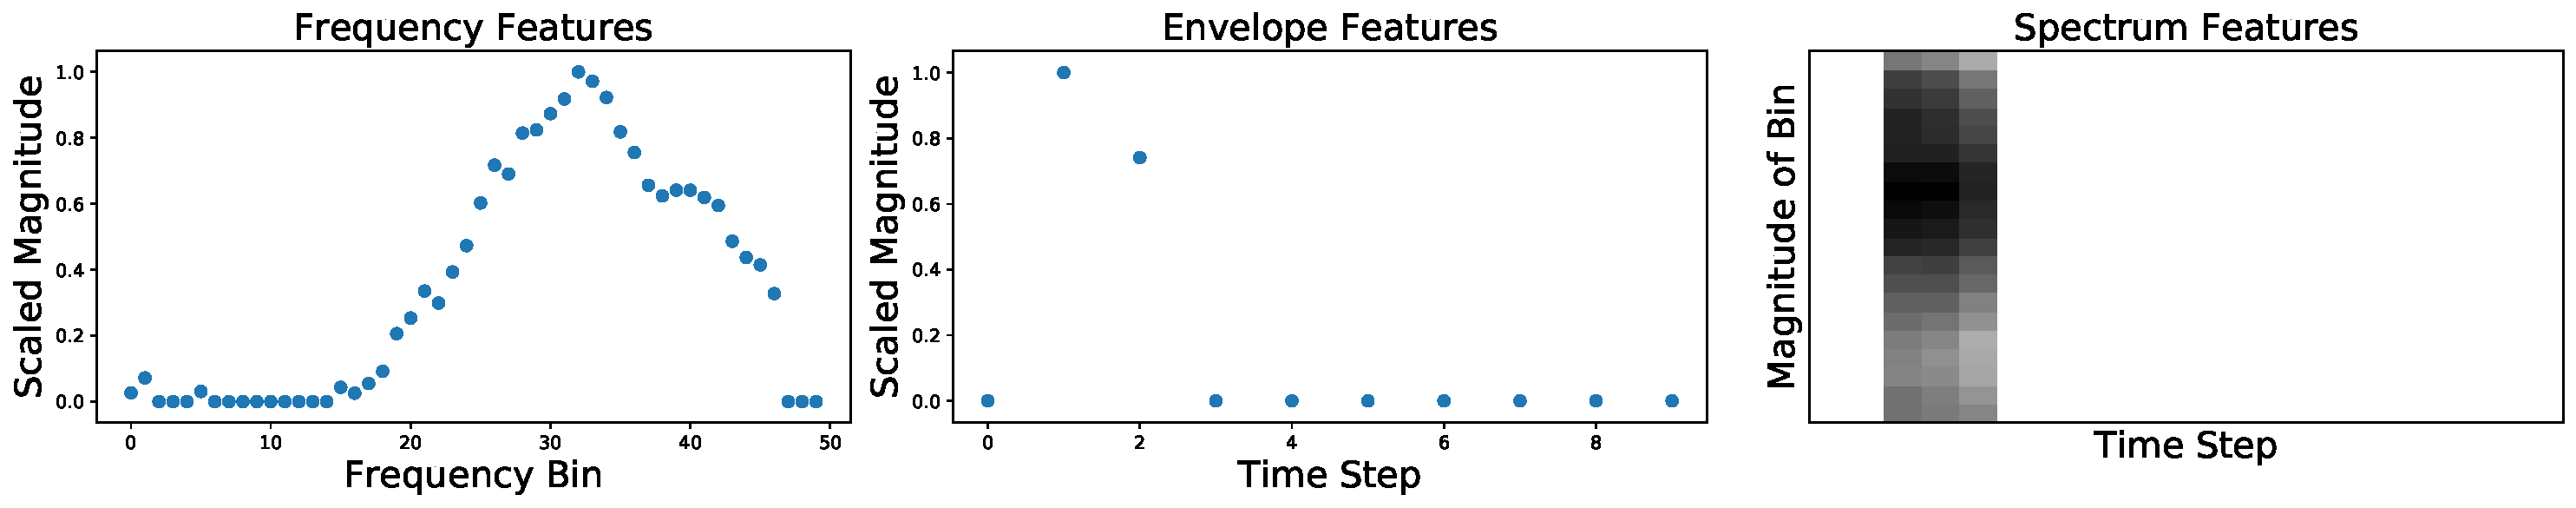
\includegraphics[width=1\columnwidth]{images/ff1.pdf}
    }
    \subcaptionbox{Randomly generated audio with percussive qualities, resembling a tight snare}{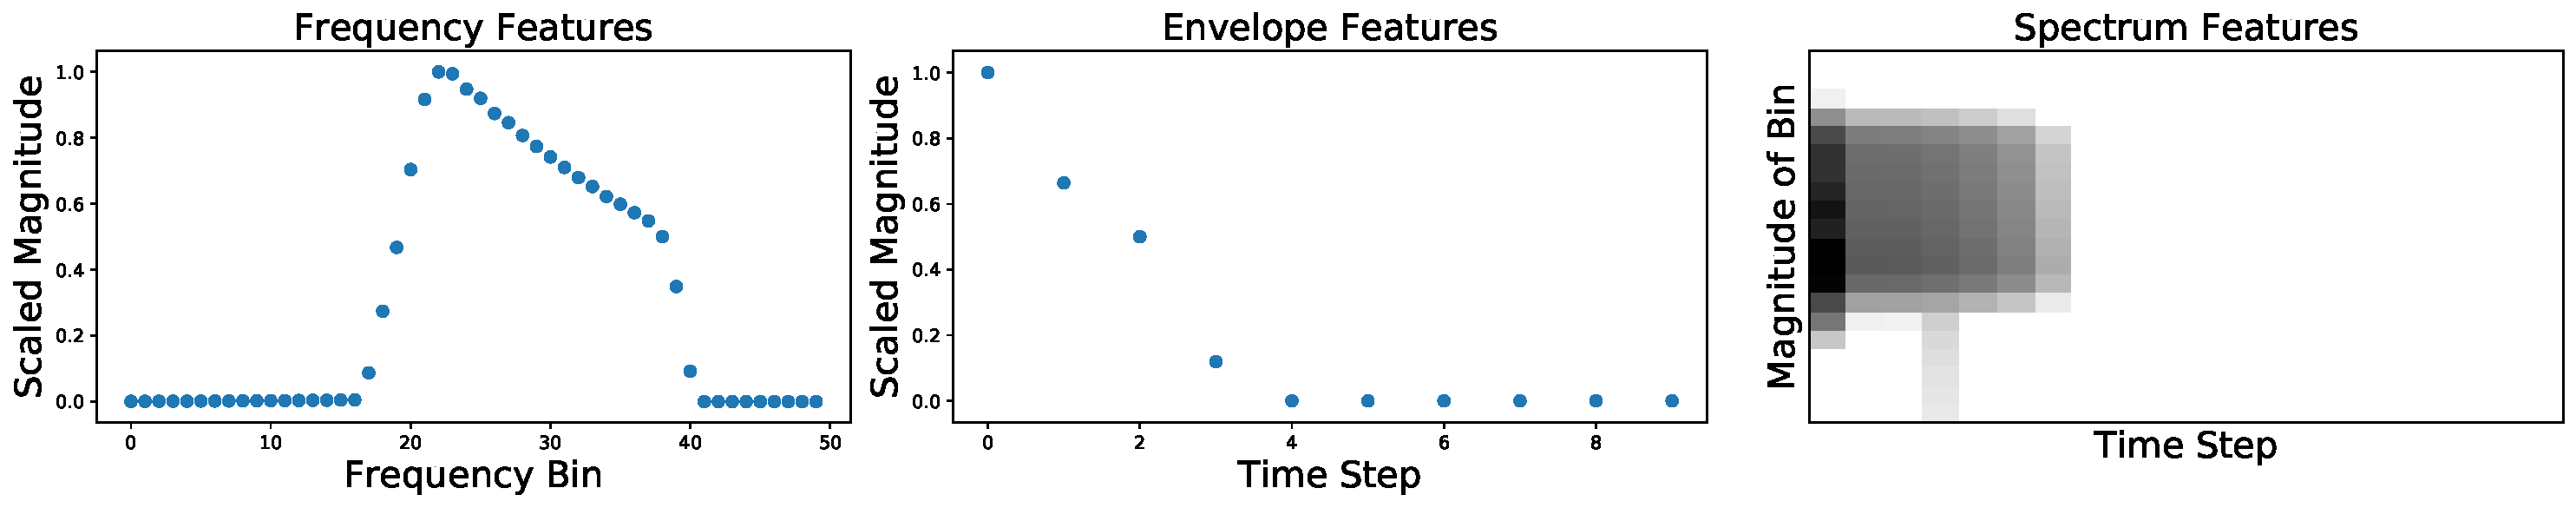
\includegraphics[width=1\columnwidth]{images/ff2.pdf}}
    \subcaptionbox{A randomly generated noise with a percussive envelop but non-percussive frequency features (modulated pitch)}
    { \includegraphics[width=1\columnwidth]{images/ff3.pdf}}
\caption{Graphed representation of features extracted for 3 different samples. }
\label{fig:stackspectrums}
\end{figure}

% \begin{enumerate}
% \item Envelope Transformation: Represents changes in loudness for the duration of the signal. Using STFT we generate a matrix $M_{i \times j}$ with rows $i$ and columns $j$ corresponding to time steps and frequency bins respectively. Values $v_{i \times j}$ indicating the magnitude of the frequency bin $j$ at each time-step $i$. Information about the envelope of the signal can be extracted by summing the values of $M$ for each time-step (or row $i$), giving us a feature vector that is normalized to the range of 0 to 1. The information contained in this vector is an alternative to Root-Mean-Square measurements of a sliding window over the signal.
% \item Frequency Transformation: A static, normalized snap-shot of the the frequencies present within the audio. The calculation of this feature vector is similar to the envelope, but the summation is done along the frequency axis. Another important distinction is that since capturing an adequate frequency resolution is important for this transformation, we utilized shorter hop-sizes and wider windows. A Mel Scale transformation was also applied in hopes that the captured features better represent human perception of frequencies. 
% \item Spectrum Transformation: This function is simply a Mel Scaled STFT with its values normalized from 0-1. Spectrograms contain more information about the original signal but their analysis requires more complex computational methods.
% \end{enumerate}

%================
\clearpage
\section{Virtual Ear Classifier Definitions}
\label{appendix:classifier_definitions}
\subsection{Two Phased models}
Using the described features, we trained several neural network models for  decision 1 and 2 with the pytorch library. The task of decision 1 is to separate drums from not-drums (DrumVsNotDrum, or DVN). The task of decision 2 is to categorize drums and percussion (DrumVsDrum, or DVD). We kept our feature space small, making it viable for feature selection and model design to be done on a trial and error basis. For all models, accuracy is calculated by prediction of all test dataset labels and the loss function and optimizer are Categorical Cross-Entropy and Adam respectively. Training continues until no reduction in loss and accuracy is observed in 10 epochs.  All activation functions are PReLU:
\begin {enumerate}
\item FC-DVN: Fully connected network trained on Envelope features, reaching 97\% accuracy on our test data for decision1. With size of 10x5x10.
\item CNNLSTM-DVN: A combination of CNN and LSTM models, where the CNN model extracts higher level features that are fed temporally to an LSTM cell. This model is trained on spectrum data and reaches 98\% accuracy on our test set. Its structure is the combination of a CNN with 2 output channels and kernel size $(7,3)$; Followed by an LSTM model of hidden size 800 and a fully connected layer of size 20x2.
\item E/F-DVD: A fully connected model trained on a concatenation of envelope and frequency features. Reaching 80\% accuracy for 5-way drum categorization in decision2. Size of 50x10x2x6.
\item CNN-DVD: A CNN model trained on Spectrum features. Reaching 82\% accuracy in a 5-way drum categorization in decision2. A combination of a CNN model with output channel size of 4, kernel of size of 5, another CNN model with output channel size of 8 and kernel of size 3. Followed by a fully connected network of shape 100x20x6.
\item FC-DVD: Fully connected 3 layer neural net with 78\% accuracy for 5-way drum categorization in decision2. Size of 400x200x50.
\end{enumerate}
Parameters are hand-picked and un-tuned. 
\subsection{Mixed Ear Models}
\label{chap3:mixed_ear_models}

 We compare the performance of our models before and after the addition of envelope features (a vector of size 10) to the feature space. We reuse the model trained on  MixedDB as our embedding feature extractor. We use a combination of RadarDB, FreeDB and NoiseDB for training. We only focus on clap,hat,kick,snares, and synthetic noise groups for measuring effectiveness to prevent class overlaps as much as possible. We also exclude samples longer than 1 second, to exclude potentially mislabeled data. Our final training database for mixed ear models is described in table~\ref{db:memDB}.

\subsubsection{Model Selection}
Using our encoding and envelope features to represent audio, five classification models were trained for the task of categorizing the five different sound groups. For hyper-parameter optimization, the models were trained using 5-fold cross validation and 80/20 train-to-test ratio. The F-Score result of each cross-validation is the unweighted average F-Score of all groups. For inter-model comparisons, the procedure is the same except 10-fold cross validations are used. Our models were derived from scikit-learn's implementations of these classifiers~\cite{pedregosa2011scikit}. Before inter-model comparisons, we conducted a grid-search for each model on at least one of its possibly decisive hyper-parameters. The classifiers and other notable specifications are presented in Table~\ref{table:mem_model_selection}. 
\begin{table}[t]
    \centering \hspace*{-0.8cm}
    \begin{threeparttable}
    \begin{tabular}[width=0.95\paperwidth]{|l|l|l|}
    \hline
    Model name & Tuned Parameters\tnote{\dag}  & Used Weights? \tnote{\ddag} \\\hline
     Support Vector Classifier (SVC) &  Gamma:0.001, C:100, kernel:rbf & Yes\\
     LinearSVC & C:10 & Yes\\
     K Nearest Neighbors & Num. Neighbors:30 &  No \\
     Random Forest Classifier & Num Estimators:500 & Yes \\
     Extra Trees Classifier & Num Estimators:1100 & Yes\\
     \hline
    \end{tabular}
    \caption{Models implemented for comparison using envelope and embedded features. }
    \begin{tablenotes}
    \item[\dag] Tuned parameters values are based on grid-searching for best f-score. Parameters not mentioned have neither been tuned nor changed from scikit-learn's default values (as of version 0.23)
    \item[\ddag] Class weights are used unless not applicable to classifier.
    \end{tablenotes}
    \label{table:mem_model_selection}
    \end{threeparttable}
\end{table}
\begin{table}[htb]
\centering
\begin{tabular}{|l|l|l|l|l|l|}
\hline
 DB Name & kick & snare & clap & hat & Synthetic Noise\\\hline
 MixedEarDB & 1334 & 1035 & 401 & 1275 & 1000 \\ \hline
\end{tabular}
\caption{A database put together by combination of RadarDB, FreeDB and NoiseDB}
\label{db:memDB}
\end{table}


\begin{figure}[htb!]
\begin{center}
    \textbf{Cross Validation F-Scores For All Sound Groups}\par\medskip
    \makebox[\textwidth]{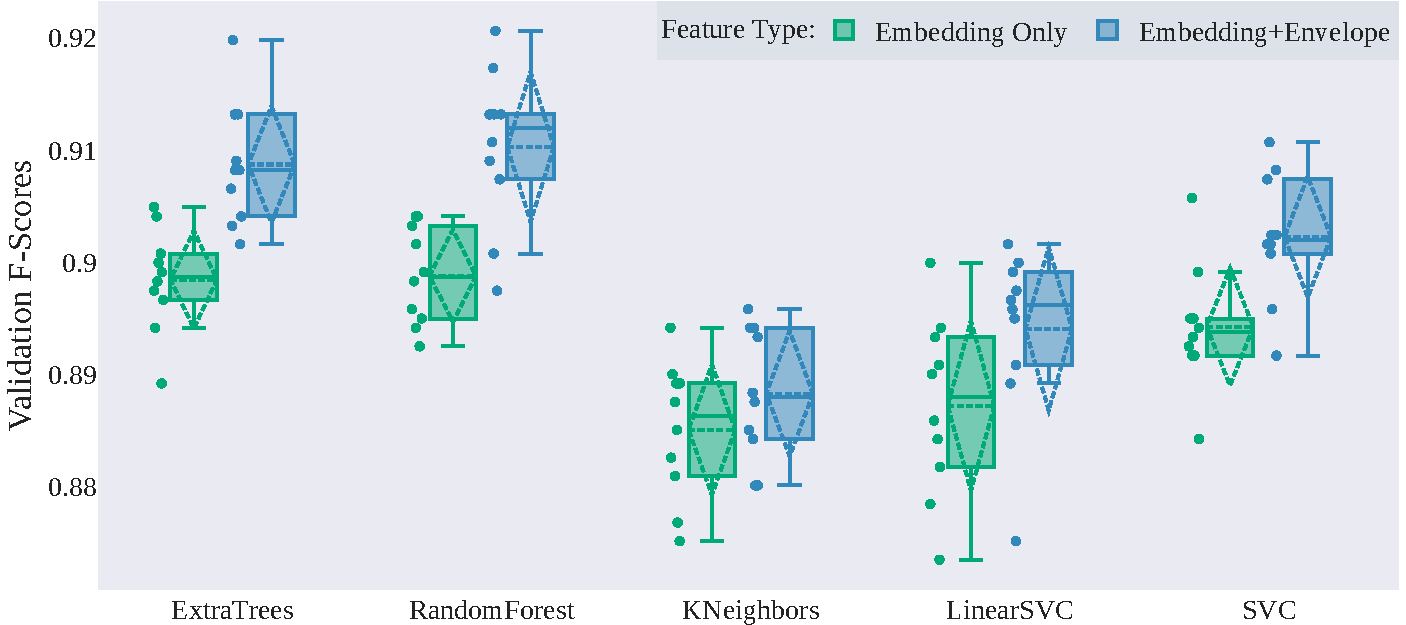
\includegraphics[width=0.7\paperwidth]{images/mme_comparisons_mme.pdf}}
    \caption{Boxplots visualizing the F-Score results for each cross-validation. The individual scores, means, medians, standard-deviation and outliers are depicted. Envelope features improve classification accuracy. }
    \label{fig:f1_allg_box}
\end{center}

\begin{center}
        \textbf{Cross Validation F-Scores For Drum Vs Not-Drum}
    \makebox[\textwidth]{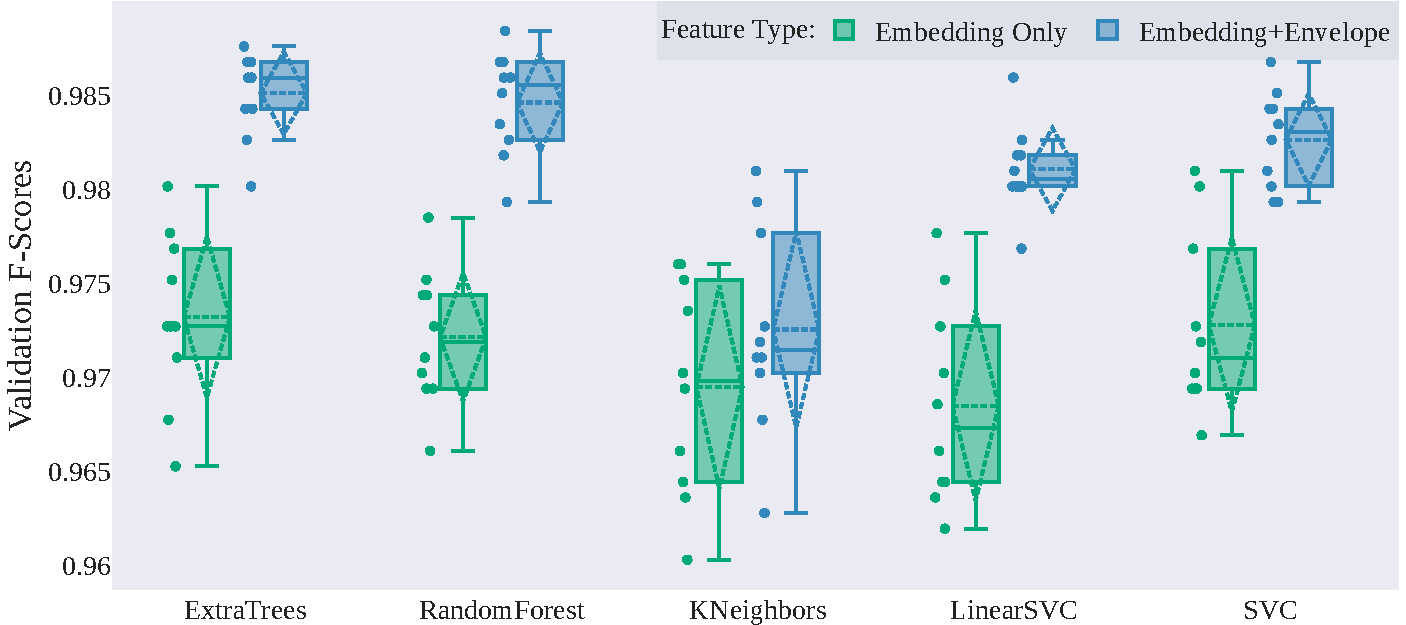
\includegraphics[width=0.7\paperwidth]{images/mme_comparisons_dvn.pdf}}
    \caption{F-Score results for each cross-validation. Models perform better as there are less categorization groups.  }
    \label{fig:f1_dvn_box}
\end{center}

\label{fig:conf_f1_dvn}
\end{figure}

% \begin{figure}[h!]
%     \begin{center}
%     \textbf{Cross Validation F-Scores For All Sound Groups}\par\medskip
%     \makebox[\textwidth]{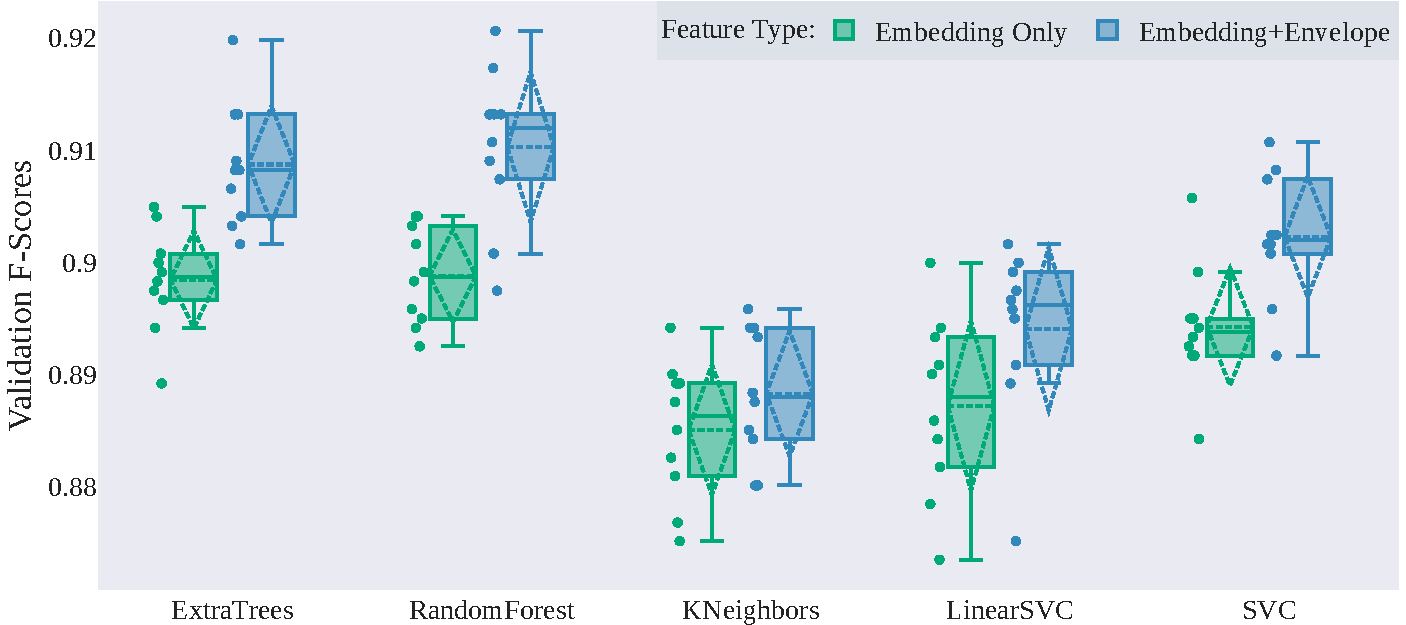
\includegraphics[width=0.8\paperwidth]{images/mme_comparisons_mme.pdf}}
%     \caption{Boxplots visualizing the F-Score results for each cross-validation. The individual scores, means, medians, standard-deviation and outliers are depicted. The differences are noticeable, yet means lie within the \%88-92 range. Envelope features improve classification accuracy for all models. }
%     \label{fig:f1_allg_box}
%     \end{center}
% \end{figure}
% \begin{figure}[h!]   
%     \begin{center}
%         \textbf{Cross Validation F-Scores For Drum Vs Not-Drum}
%     \makebox[\textwidth]{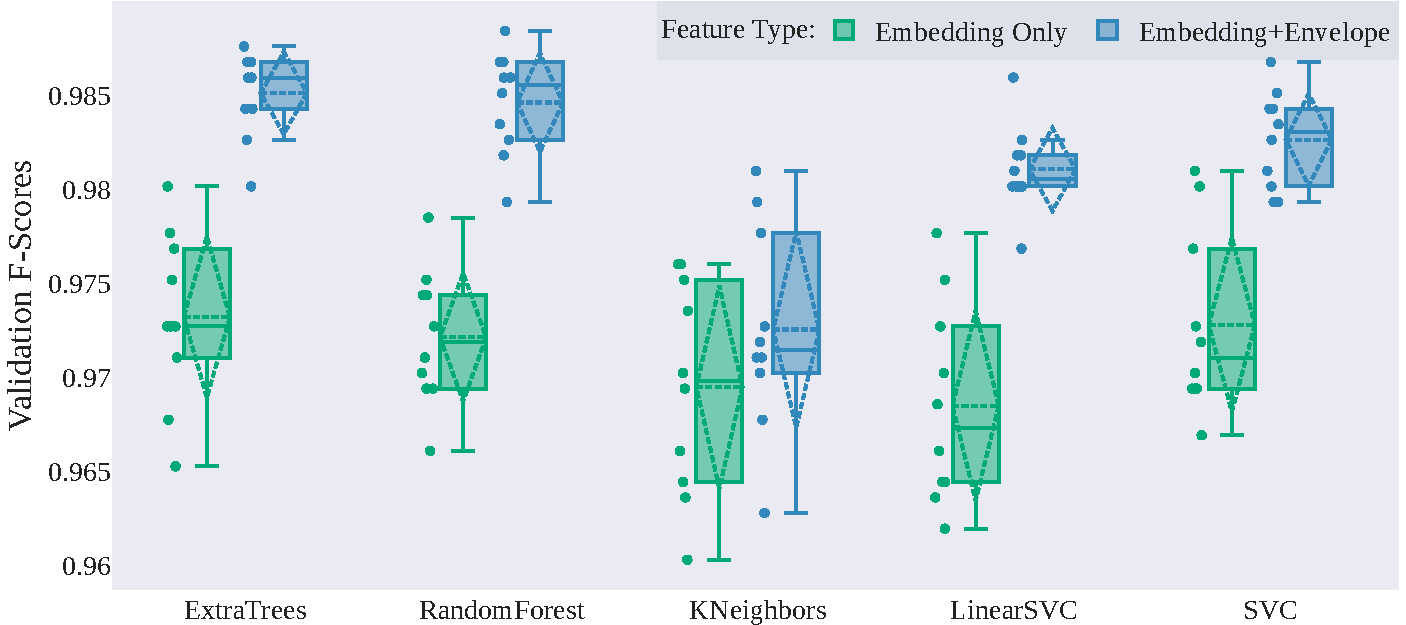
\includegraphics[width=0.8\paperwidth]{images/mme_comparisons_dvn.pdf}}
%     \caption{F-Score results for each cross-validation. Models perform better as there are less categorization groups. Envelope features increase accuracy for all models. Random Forest and Extra Trees remain the top two models. }
%     \label{fig:f1_dvn_box}
%     \end{center}
% \end{figure}
% We're also interested in how these models perform on the binary drum vs not drum task.
% After grouping all drums together, we repeat the model selection process above. We also repeat the hyper-parameter optimization step where no changes appeared necessary except for a reduction in the number of neighbors for the K-Neighbor model (from 30 to 5). As show in in Figures~\ref{fig:f1_allg_box} and~\ref{fig:f1_dvn_box}, the addition of envelope features had a positive effect on performance for all mdoels, yet the RandomForest and ExtraTrees models clearly outperform the other classifiers in both tasks. We train the top two models on \%80 of our database and use the remaining \%20 to create the confusion matrices and the F-Scores shown in Figures~\ref{fig:conf_f1_dvn}.



\begin{figure}[htb!]
\begin{center}
    \textbf{ Classification Report for DvDvN and DvN  }\par\medskip
    \makebox[\textwidth]{
    \subfloat[Precision, recall, F1-Score, and number of supporting examples]{ 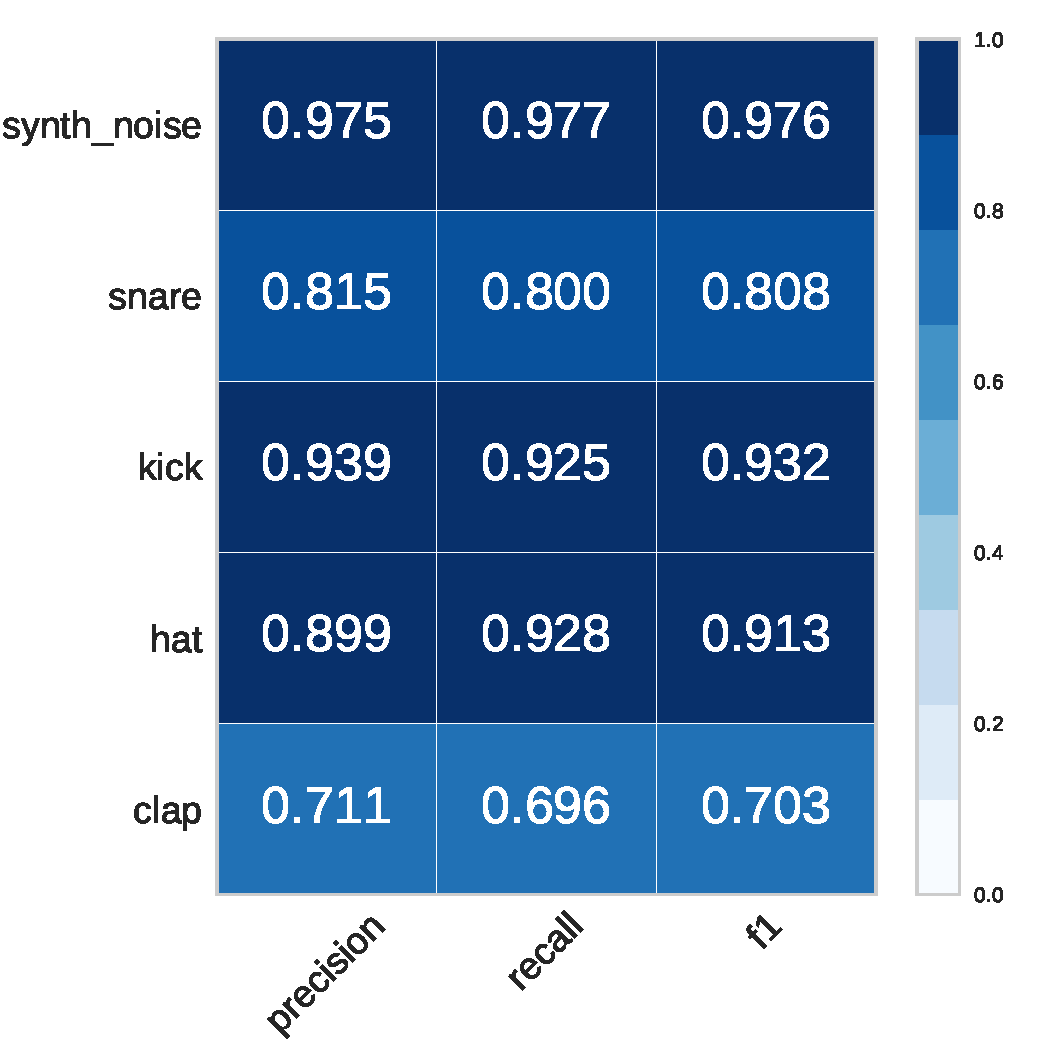
\includegraphics[width=7cm,height=7cm]{images/f1_mme.pdf}
    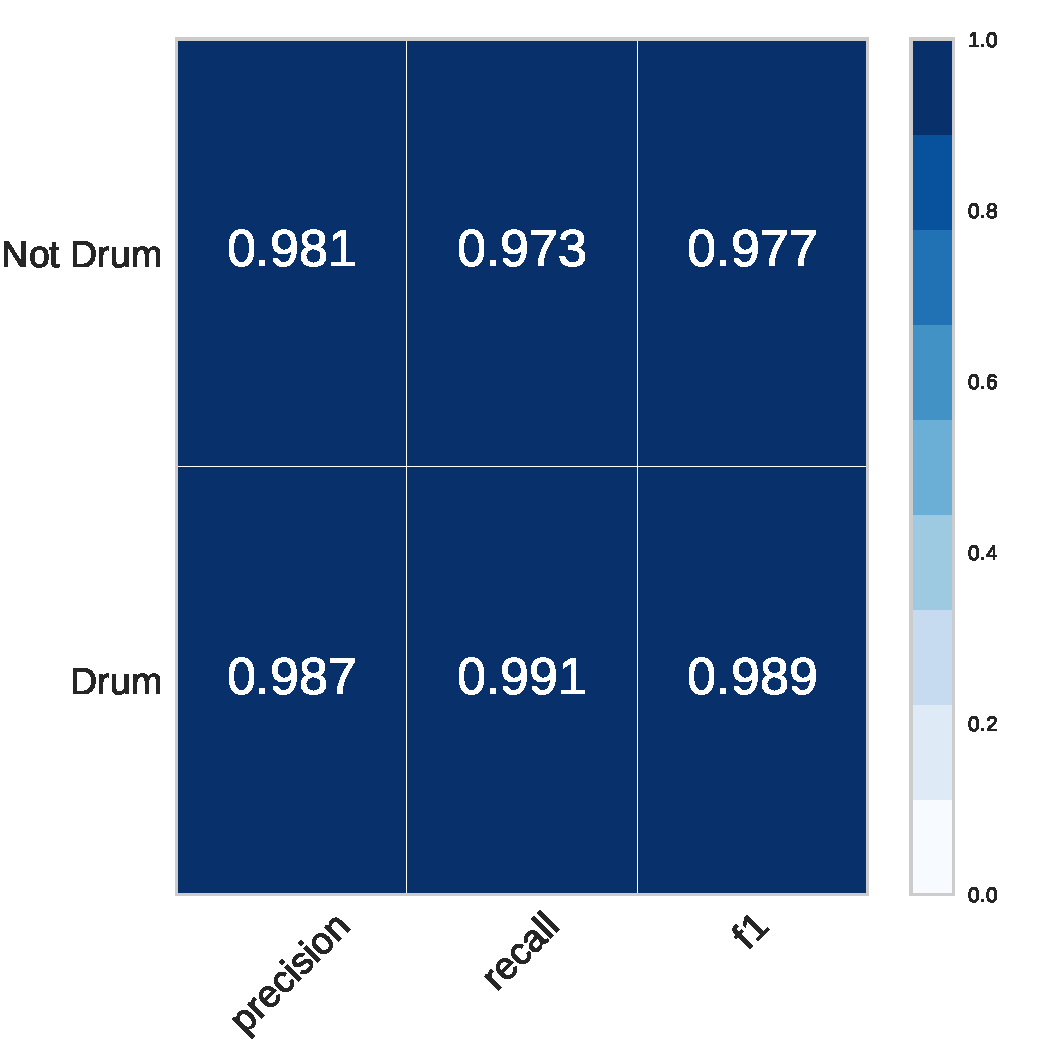
\includegraphics[width=7cm,height=7cm]{images/f1_dvn.pdf}
    }
    
    }
\label{fig:conf_f1_dvd}
\end{center}

\begin{center}
    \makebox[\textwidth]{
    \subfloat[Confusion matrices]{ 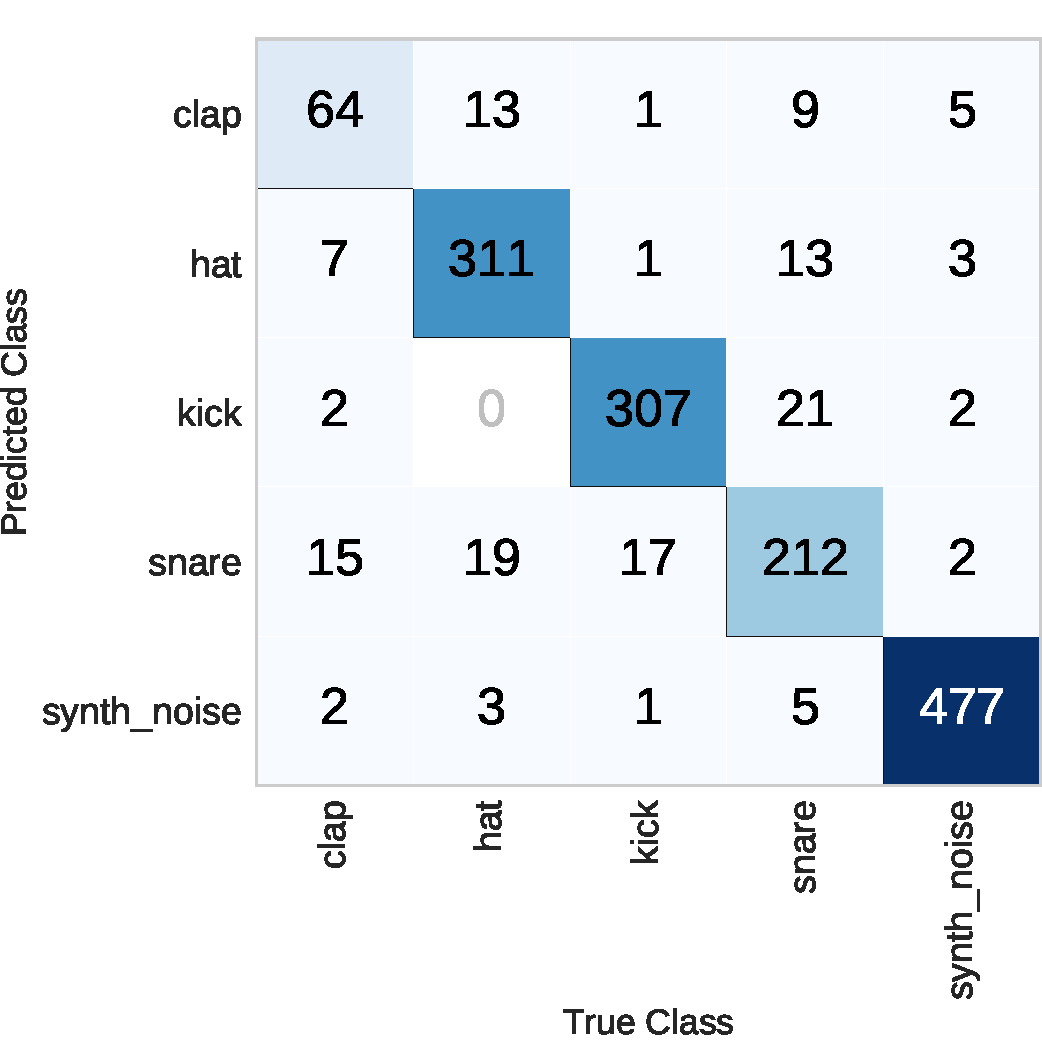
\includegraphics[width=7cm,height=7cm]{images/conf_mme.pdf}
    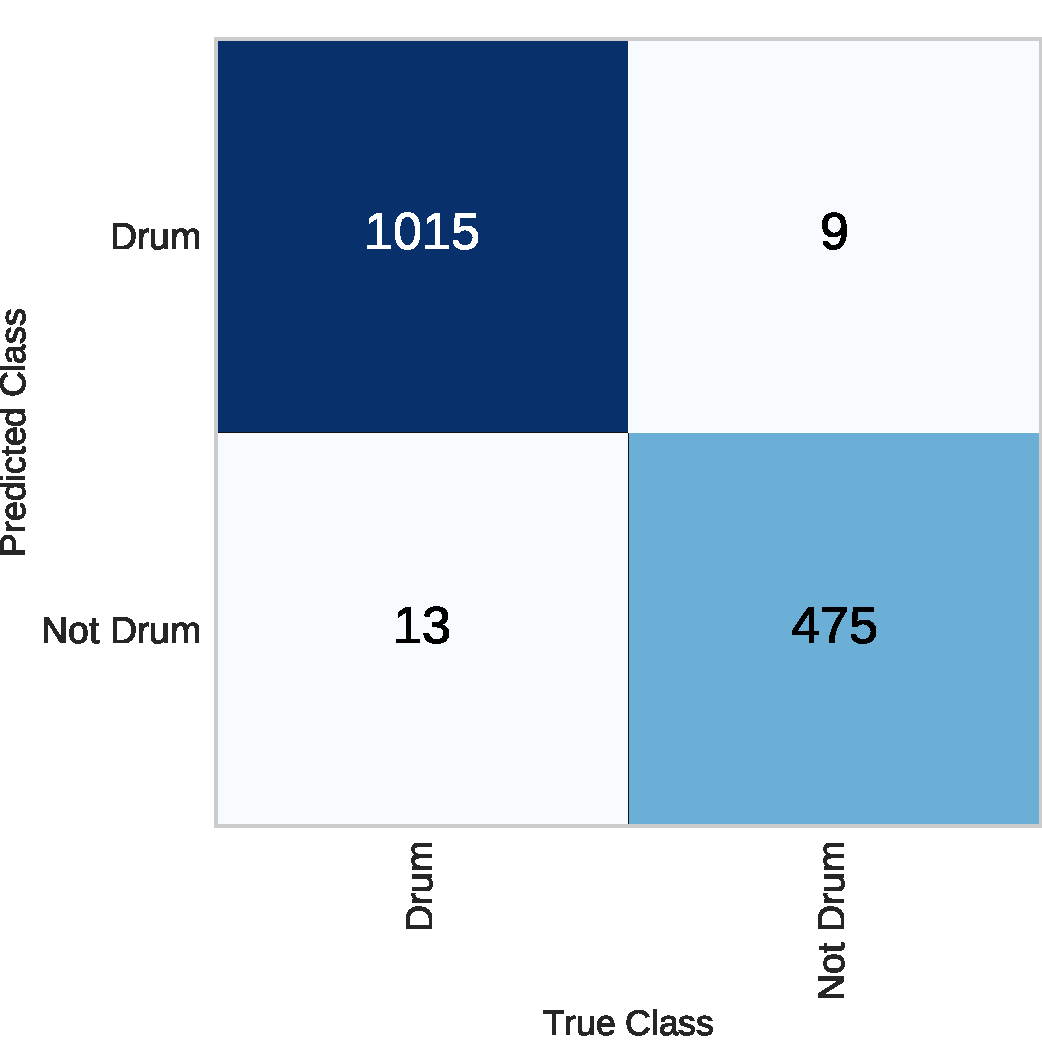
\includegraphics[width=7cm,height=7cm]{images/conf_dvn.pdf}
    }}
\end{center}
\caption{F-Scores and confusion matrix of ExtraTrees model for both DvDvN and DvN.}
\label{fig:conf_f1_dvn}
\end{figure}

% Based on these reports, having multiple options for drum categorization does not noticeably influence our models accuracy in categorizing synthetic noise as synthetic noise. However, the DvDvN models's slightly smaller false negative rate for synthetic noise (11 vs 13 false negatives) is countered by a slightly higher rate of categorizing drums as synthetic noise (12 vs 9).  We therefore use the DvDvN implementation as it simultaneously categorizes drum types and separates noise from drums. However, without manual inspection, we cannot confirm the extent of this model's usefulness. 
%==============
\clearpage
\section{AutoEncoder Structures and Hyper-Parameter Optimization}
\label{appendix:hyperparam}
% could do multi-objective pareto front stuff too
Within the context of machine learning, a model's \emph{hyper-parameters} are fixed parameters which are set before the training begins (e.g number of layers, size of layers, loss function) and are not learned during the minimization procedure~\cite{bengio2000gradient}. To assist us with the construction of our model, we defined a number of possible choices for the architecture of our model and audio-transformers and used hyper-parameter optimization to extract promising sets of values~\ref{table:hyper_params}. 

The list of possible choices for the selected hyper-parameters can be found in table~\ref{table:hyper_params}. We included not only model parameters but also spectrogram transformation parameters within this search space, as GPU accelerated FFT calculations allows ad hoc audio transformations to take place parallel to the training process. We implemented 3 base models which are affected by these hyper-parameters. The \enquote{Model Type} parameter dictates whether CNN or fully connected models are selected; If a \enquote{fully connected} model is selected, the \enquote{hidden layers} parameter selects between the two implementations. The specifications for these models can be found in tables~\ref{table:FC1_AUTOENCODER},~\ref{table:FC2_AUTOENCODER} and~\ref{table:CNNAUTOENCODER}.

Using the optuna optimization tools \cite{akiba2019optuna}, we conducted 500 search trials. The trial's success is measured in their final loss value, calculated by applying the model to the test data-set. Each trial consisted of 20 epochs of training.

\begin{table}[b!]
\centering
\begin{tabular}{|p{6cm}|p{6cm}|}
\hline
Hyper-Param. & Value  \\ \hline
Model Type      &  CNN  \\ \hline
Optimizer       & Adam  \\ \hline
Hidden Layers   & Not Applicable  \\\hline
Learning Rate   &  0.001145\\ \hline
Frequency Bins & 30 \\ \hline
Time Steps & 20 \\ \hline
Latent Size & 64 \\ \hline
Regularization & 3.25^{-6}\\ \hline
Dropout Rate & 0.5 \\ \hline
\end{tabular}
\caption{Top performing hyper-parameter set}
\label{table:best_params}
\end{table}
\begin{table}[htb]
\begin{tabular}{|p{28mm}|p{50mm}|p{21mm}|p{21mm}|}
\hline
Hyper-Param. & Description  & Values & Distribution\\ \hline
Model Type      &   Affects encoder's first hidden layer & CNN,FC & Categorical \\  \hline
Optimizer       & Updates network's weights based on loss & Adam,SGD & Categorical  \\  \hline
Hidden Layers   & Extra hidden layer for the Encoder & True,False & Categorical \\  \hline
Time Steps & Temporal granularity of the spectrogram. Affects FFT windowing. & 10,20 & Categorical  \\ \hline
Learning Rate   &    Optimizer's learning rate  & $1^{-4}$ ... $1^{-1}$ & Uniform      \\ \hline
Frequency Bins & Number of spectrogram frequency bins & 10, 30,60 & Categorical \\ \hline

Regularization  &  L2 regularization parameter. Penalizes large weights to prevent overfitting & 1^{-6}~...~1^{-1} & Uniform\\ \hline
Latent Size & Size of bottle neck layer or number encoded features & 8,16,64 & Categorical              \\ \hline
Dropout Rate & Random zeroing of activations between layers to prevent over-fitting & 0,0.5,0.1 & Categorical\\  \hline
\end{tabular}
\caption{The Hyper-Paramter space in which the optimization was conducted.}
\label{table:hyper_params}
\end{table}
\begin{table}
\begin{tabular}{|p{3cm}|p{3cm}|p{3cm}|p{3cm}|}
\hline
Layer-\# & Out Shape & Param Num & Details  \\ \hline
Conv2d-1 & [-1, 8, 30, 20] &   208 & Encoder's input \newline
Num. Channels:8\newline
kernel:5x5\newline                  
stride:1\newline    
padding:2 \\ \hline
ReLU-2 & [-1, 8, 30, 20] &   0 & \\  \hline
MaxPool2d-3 & [-1, 8, 15, 10] & 0 &  kernel:5x5 \newline
stride:2 \\ \hline
Dropout-4 & [-1, 8, 15, 10] & 0 &  \\ \hline
Linear-5 & [-1, 8] & 9,608 & Encoder's output \\ \hline
Linear-6 & [-1, 256] & 2,304 & Decoder's Input \\ \hline
Dropout-7 & [-1, 256] & 0 &  \\ \hline
Linear-8 & [-1, 600 ] &  154,200& Decoder's output\\ \hline
\end{tabular}
\caption{CNN model design with latent size of 8. 30 and 20 are the assumed frequency bins and step size. Total number of parameters is 166,320. }
\label{table:CNNAUTOENCODER}
\end{table}

\begin{table}
\begin{tabular}{|p{3cm}|p{3cm}|p{3cm}|p{3cm}|}
\hline
Layer-\# & Out Shape & Param Num & Details  \\ \hline
Linear-1 & [-1, 128]  & 76,928 & Encoder's input \\ \hline
Dropout-2 & [-1, 128] & 0 &  \\ \hline
Linear-3 & [-1, 8] & 9,608 & Encoder's output \\ \hline
Linear-4 & [-1, 128] & 2,304 & Decoder's Input \\ \hline
Dropout-5 & [-1, 128]  & 0 &  \\ \hline
Linear-6  & [-1, 600 ] &  77,400 &Decoder's output\\ \hline
\end{tabular}
\caption{Fully connected model with only 1 hidden dimension for encoder and decoder. Designed assumes latent size of 8. 30 and 20 are the assumed frequency-bins and step-size values. Total number of parameters is 156,512.}
\label{table:FC1_AUTOENCODER}
\end{table}

\begin{table}

\begin{tabular}{|p{3cm}|p{3cm}|p{3cm}|p{3cm}|}
\hline
Layer-\# & Out Shape & Param Num & Details  \\ \hline
Linear-1 & [-1, 128]  & 76,928 & Encoder's input \\ \hline
Dropout-2 & [-1, 128] & 0 &  \\ \hline
Linear-3 & [-1, 32]  & 4,128 & \\ \hline
Dropout-4 & [-1, 128] & 0 &  \\ \hline
Linear-5 & [-1, 8] & 9,608 & Encoder's output \\ \hline
Linear-4 & [-1, 32] & 2,304 & Decoder's Input \\ \hline
Dropout-5 & [-1, 32]  & 0 &  \\ \hline
Linear-4 & [-1, 128] & 2,304 & \\ \hline
Dropout-5 & [-1, 128]  & 0 &  \\ \hline
Linear-6  & [-1, 600 ] &  77,400 &Decoder's output\\ \hline
\end{tabular}
\caption{Fully connected model with 2 hidden dimensions for encoder and decoder. Designed assumes latent size of 8. 30 and 20 are the assumed frequency-bins and step-size values. Total number of parameters is 163,232.}
\label{table:FC2_AUTOENCODER}
\end{table}

% \begin{figure}[htb]
% \centering
% \textbf{Tracing the Best Loss Values}
% 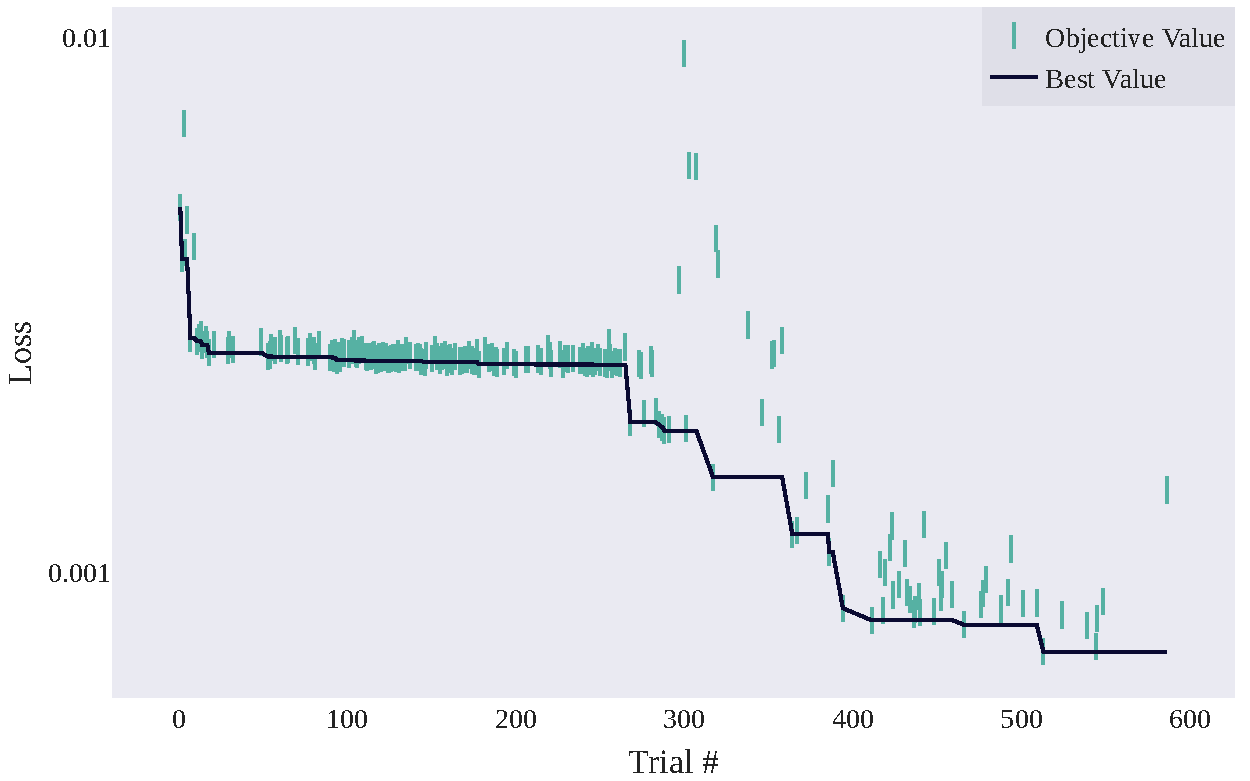
\includegraphics[width=12cm,height=7cm]{images/Optimization_History.pdf}
% \caption{Best loss values found during hyper-parameter optimization. The effect of a switch to random sampling and an increase of the pruning threshold can be observed during trials 270 and 310.}
% \label{chap3:bestvalues}
% \end{figure}

\begin{figure}[tb]
\begin{center}
    \textbf{Hyper-Parameters' Loss Correlation}
    \makebox[\textwidth]{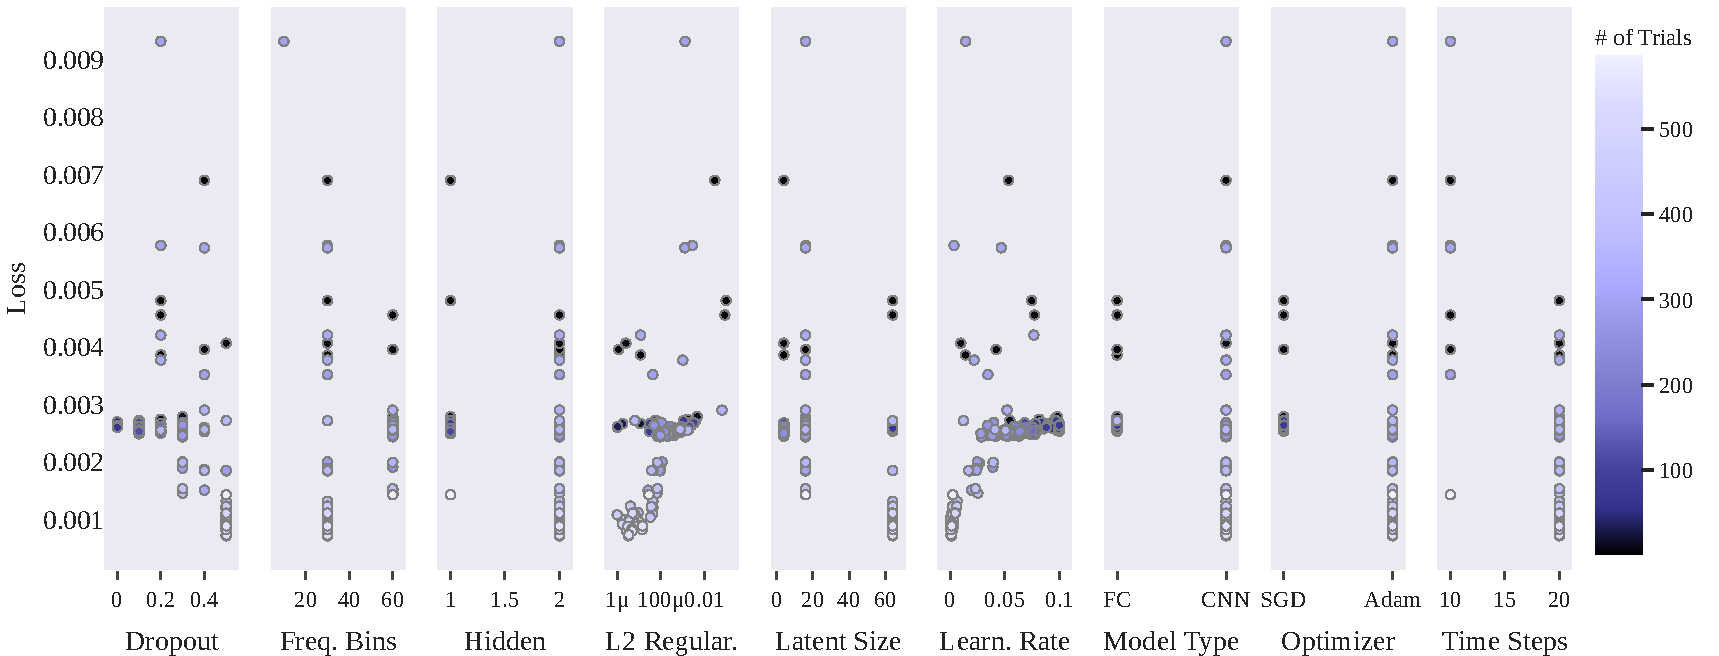
\includegraphics[width=0.85\paperwidth]{images/slice_plot.pdf}}
      \caption{Sliced plot depicting the correlation between hyper-parameters and loss values. The color-scale shows the number of times each parameters has been used in a trial. Our sampling algorithm aims to utilize spaces with higher potential more often. }
    \label{fig:slicegraph}
    \end{center}
\end{figure}




%==============
% \chapter{Embedded Feature Visualization}
% Live demos provided in project source code.
% \label{appendix:tsne}
% \begin{figure}[]
% \centering
% \textbf{2 Dimensional Projection of Latent Variables}\par\medskip
%  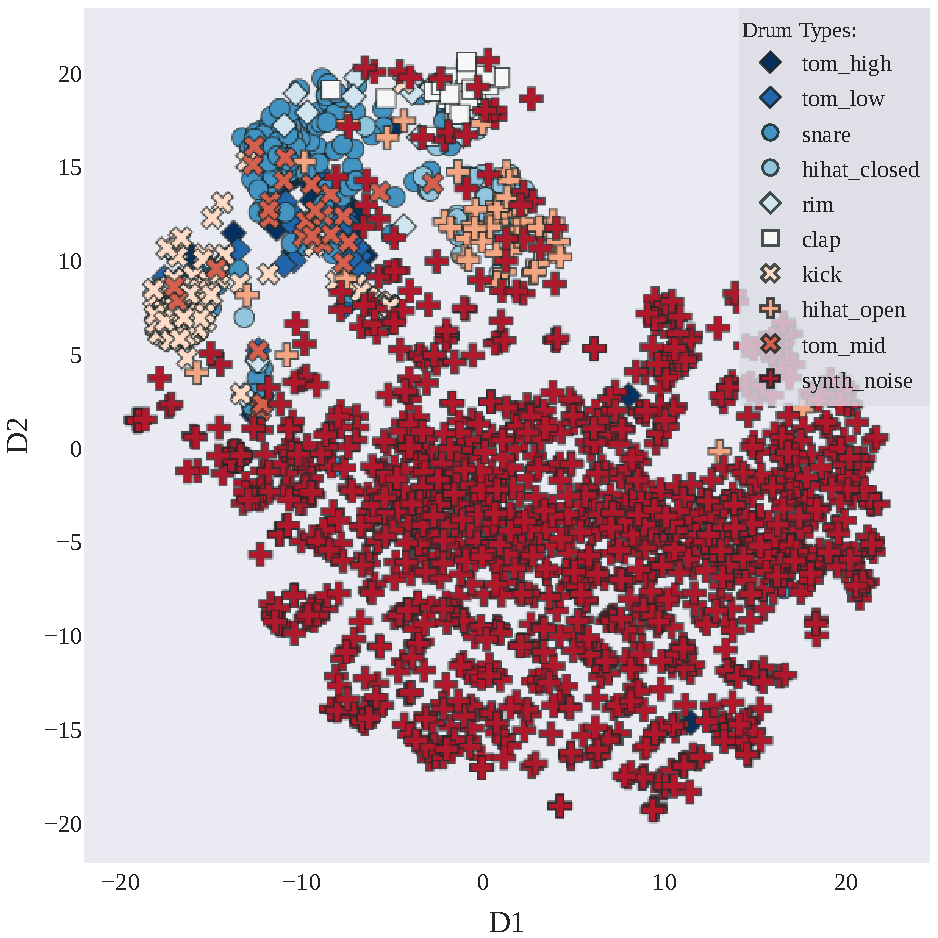
\includegraphics[width=0.90\linewidth]{images/t-SNE_2d.pdf}
% \caption{Projection of an embedding model's low dimensional encoding on to a 2D plane. We implemented interactions for these graphs for manual inspection of samples. }
% \label{fig:2d_tsne}
% \end{figure}

% \begin{figure}[]
% \centering
% \textbf{3D t-SNE Projection}\par\medskip
% \mbox{\subfloat[]{\label{subfig:1} \fbox{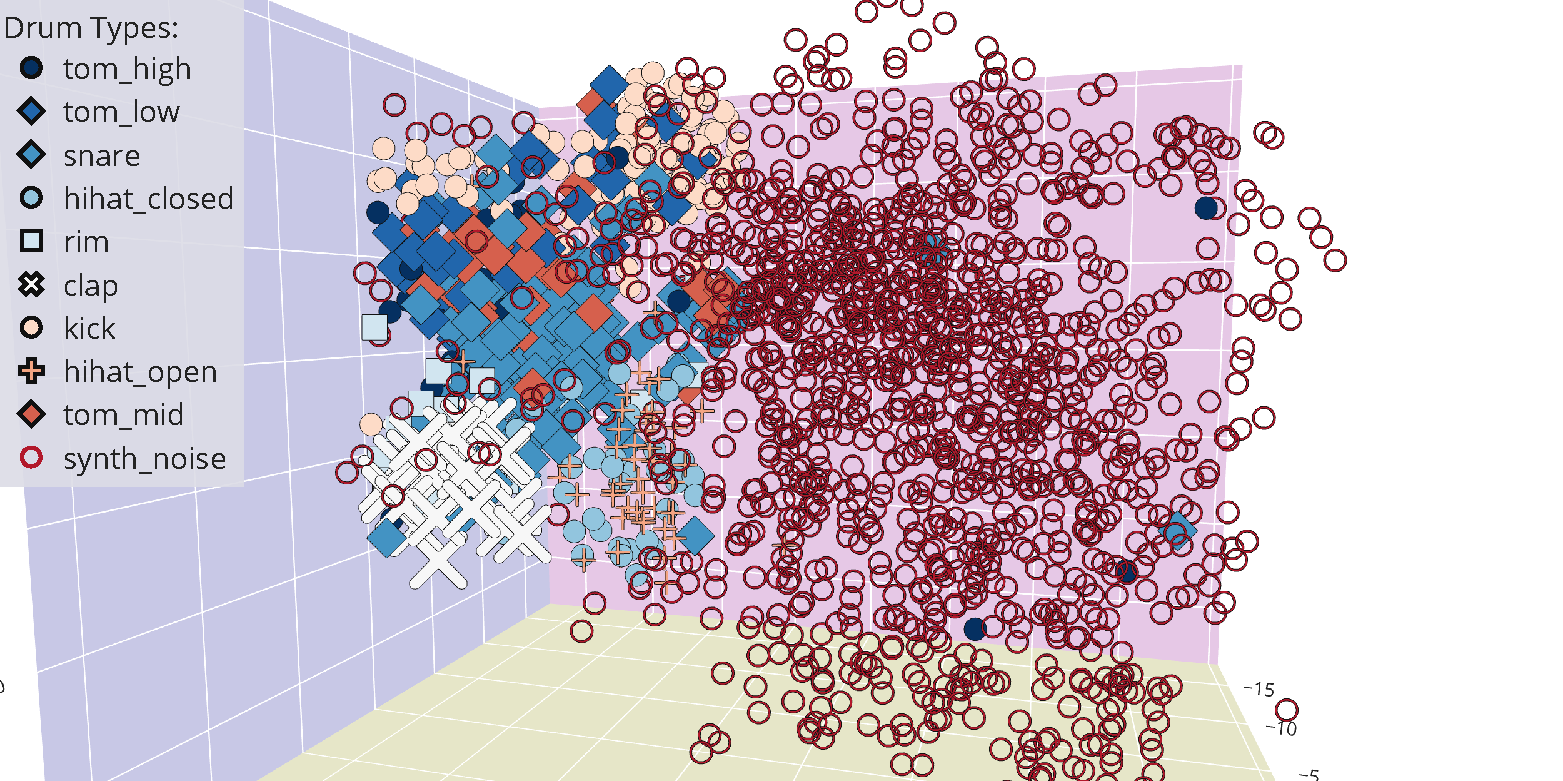
\includegraphics[width=12cm,height=6.8cm]{images/3d_t-SNE_symdrum_type_cam0.pdf}}}}

% \mbox{\subfloat[]{\label{subfig:2} \fbox{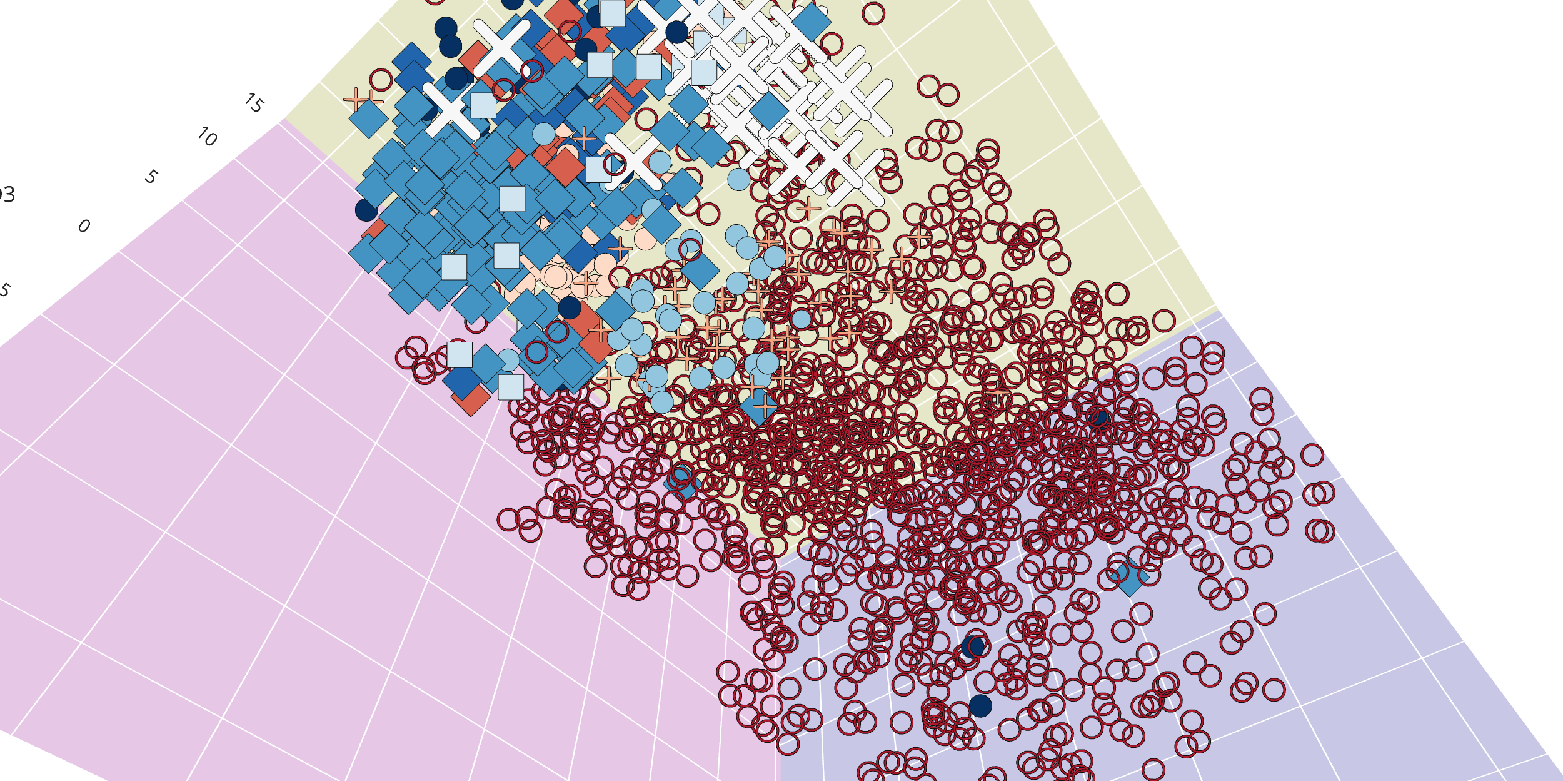
\includegraphics[width=12cm,height=6.8cm]{images/3d_t-SNE_symdrum_type_cam3.pdf}}}}

% \fbox{\mbox{\subfloat[]{\label{subfig:2} 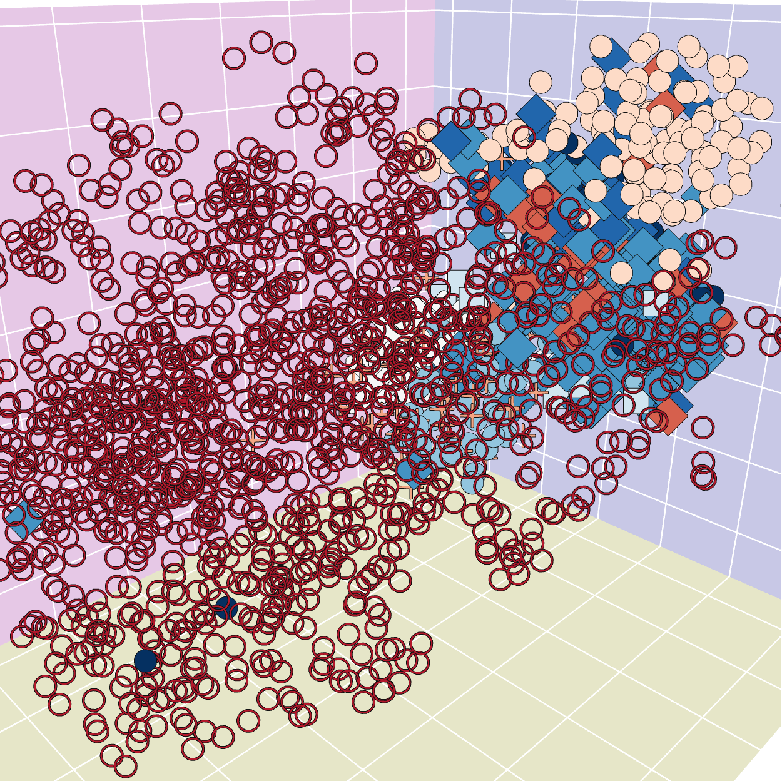
\includegraphics[width=6cm,height=6cm]{images/3d_t-SNE_symdrum_type_cam1.pdf}}}
% \mbox{\subfloat[]{\label{subfig:2} 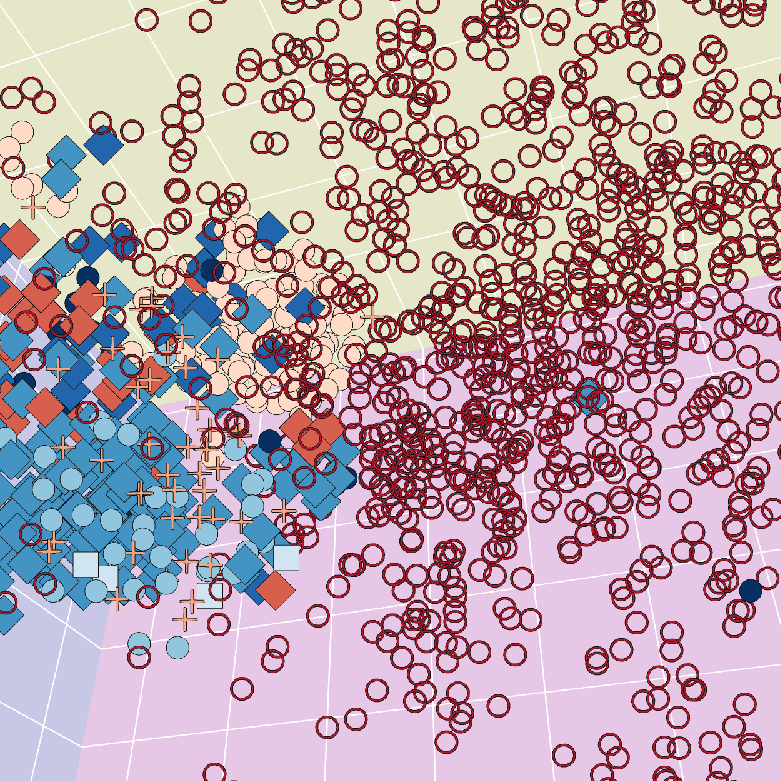
\includegraphics[width=6cm,height=6cm]{images/3d_t-SNE_symdrum_type_cam2.pdf}}}}
% \caption{3D projections of the data used for Figure~\ref{fig:2d_tsne}. Interactive demos are also implemented for 3D projections.}
% \label{fig:3d_tsne}
% \end{figure}


% %==============
\clearpage
\section{Survey Details}
\label{appendix:surveys}
Details of survey responses are presented in figures~\ref{fig:freq-survey-2p} and~\ref{fig:freq-survey-mme}. The surveys were done blinded with the two authors assigning categories to unlabled sounds.
% \begin{table}[h!]
%   \begin{tabular}{|c | c | c | c | c | c | c|} 
%   \hline
%   Drop Rule & Size & H+H & H+FC & H+CNN & H+E/F & 3 models \\ [0.5ex] 
%   \hline
%   No Drops & 257 &0.37 & 0.35 & 0.36 & 0.36 & 0.28\\ 
%   \hline
%   Assigned \enquote{Bad} By Both & 236 & 0.31 & 0.37 & 0.37 & 0.38 & 0.30 \\
%   \hline
%   Assigned \enquote{Bad} By Either & 180 & 0.47 & 0.50 & 0.48 & 0.48 &  0.34 \\
%   \hline
%   Assigned \enquote{Bad} or \enquote{Other} By Either & 154 & 0.47 & 0.59 & 0.54 & 0.50 &  0.35 \\
%   \hline
%  \end{tabular}
%  \caption{\label{kappa_table_TPE}Table of Fleiss' kappa coefficient to measure the degree of agreement between persons (H+H), persons with FC model (H+FC), persons with CNNLSTM model, persons with all models (H+E/F), and between the 3 models. } % AH: Which decision is this?
%  \end{table}
% \begin{table}[h!]
%  \begin{tabular}{|c| p{2cm} | p{2cm}| p{2cm}|} 
%  \hline
%  Drop Rule & Size & H+H & H+MEM \\
%  \hline
%  No Drop & 300 & 0.34 & 0.25\\ 
%  \hline
%  Assigned Bad By Both & 249 & 0.20 & 0.26 \\
%  \hline
%  Assigned Bad By Either & 151 & 0.46 &  0.47 \\
%  \hline
% Assigned \enquote{Bad} or \enquote{Other} By Either  & 120 & 0.62   &  0.59 \\
%  \hline
% \end{tabular}
% \caption{\label{kappa_table_MEM}Table of Fleiss' kappa coefficient to measure the degree of agreement between persons (H+H) and persons with MEM (H+MEM).}
% \end{table}
\begin{figure}[h!]
    \begin{center}
    \textbf{Category Assignment Frequency For TPE Survey}
    \makebox[\textwidth]{
    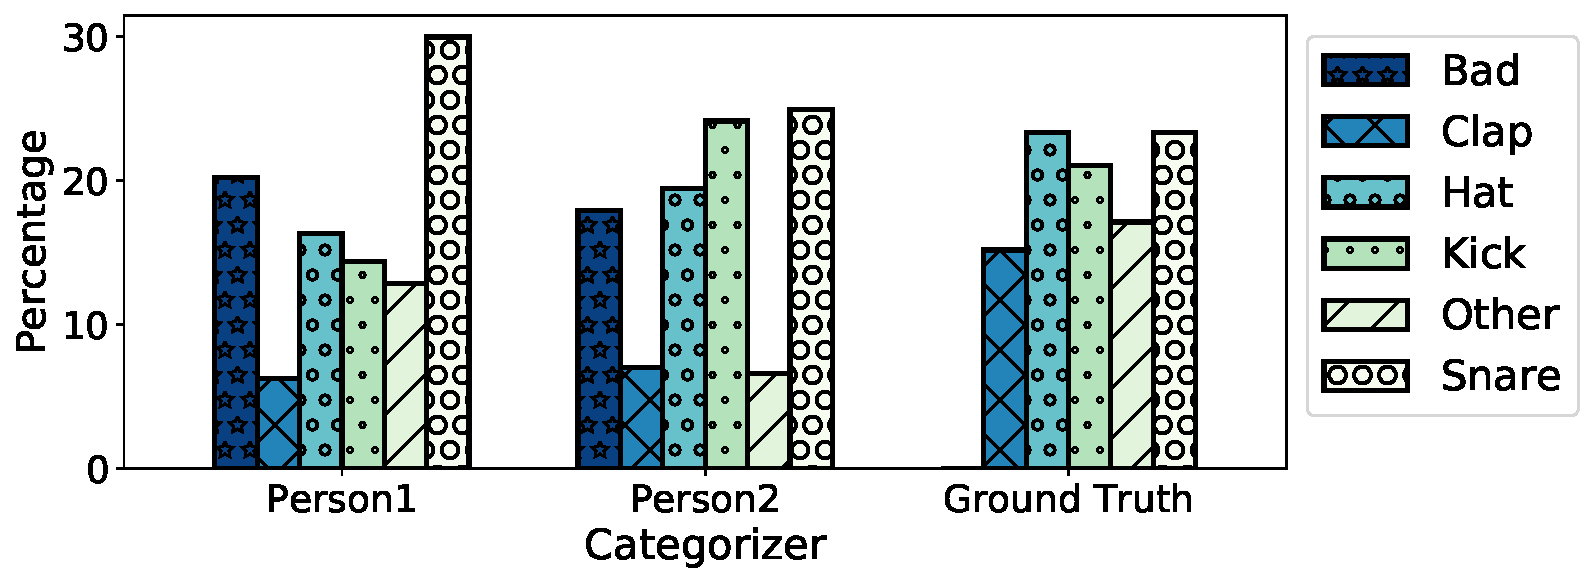
\includegraphics[width=1.1\linewidth]{images/cat_2p.pdf}}
    \end{center}
    \caption{Frequency of assigned labels by persons vs the true number of labels}
\label{fig:freq-survey-2p}
\end{figure}

\begin{figure}[h!]
    \begin{center}
    \textbf{Category Assignment Frequency For MEM Survey}
    \makebox[\textwidth]{
    \includegraphics[width=1.1\linewidth]{images/cat_MME.pdf}}
    \end{center}
    \caption{Frequency of assigned labels by persons vs the true number of labels}
\label{fig:freq-survey-mme}
\end{figure} 
\end{appendices}
\end{document}
